% \clearpage
\setcounter{page}{1}
\setcounter{section}{0}
\setcounter{figure}{0}
\setcounter{table}{0}
% \maketitlesupplementary


\renewcommand{\thesection}{\Alph{section}}
\renewcommand{\thetable}{S\arabic{table}}
\renewcommand{\thefigure}{S\arabic{figure}}


%%%%%%%%%%%%%%%%%%%%%%%%%%%%%%%%%
% \renewcommand{\contentsname}{}
% \tableofcontents

\noindent Our Supplementary Material consists of 7 sections: 


\begin{itemize}[leftmargin=2.0em]
    \item Section~\ref{sec:supp_implement} provides a detailed statement of our experiments, including the implementation details of comparison methods, and details of our test set.
    \item Section~\ref{sec:supp_eval} provides a detailed statement of our evaluation, including the details of evaluation metrics, and details of the user study.
    \item Section~\ref{sec:supp_extend_comp} adds more comparison experiments, including the comparison with StyleDrop, comparison in multi-reference stylized image generation, and comparison with style transfer methods.
    \item Section~\ref{sec:supp_extend_ablation} adds additional ablation study on different adapter architecture.
    \item Section~\ref{sec:supp_app} explores the extended application of StyleCrafter, including the collaboration with depth control.
    \item Section~\ref{sec:supp_more_result} demonstrates more results of our methods.
    \item Section~\ref{sec:supp_limitation} discusses the limitations.
\end{itemize}

% In addition to this supplementary document, we highly encourage readers or reviewers to explore our \textbf{local HTML webpage for video comparisons}. This resource provides a more interactive and visual insight, facilitating in-depth comprehension about StyleCrafter's advantages and limitations.

%%%%%%%%%%%%%%%%%%%%%%%%%%%%%%%%%
\section{Implementation Details} 
\label{sec:supp_implement}

\subsection{Comparison methods}

For all comparison methods, we follow the instructions from the official papers and open-source implementations. Since some methods including Dreambooth and InST require additional finetuning, we provide all implementation details as follows:

\paragraph{Dreambooth} \label{sec:supp_train_dreambooth} Dreambooth~\cite{dreambooth} aims to generate images of a specific concept (e.g., style) by finetuning the entire text-to-image model on one or serveral images. We train Dreambooth based on Stable Diffusion 1.5. The training prompts are obtained from BLIP-2~\cite{li2023blip2}, and we manually add a style postfix using the rare token "sks". For example, "two slices of watermelon on a red surface in sks style" is used for the first style reference in Table~\ref{tab:supp_style_ref}. We train the model for 500 steps for single-reference styles and 1500 steps for multi-reference styles, with learning rates of $5 \times 10^{-6}$ and a batch size of $1$. The training steps are carefully selected to achieve the balance between text alignment and style conformity. 

% \paragraph{CustomDiffusion} CustomDiffusion~\cite{customdiffusion} propose an efficient method for fast tuning text-to-image models for certain styles or concepts. We train CustomDiffusion based on Stable Diffusion 1.5. Similar to Dreambooth, we obtained training prompts from BLIP-2~\cite{li2023blip} and we manually add postfix like "in <new1> style". We generate a set of 200 regularization images from mannually designed instant prompts for each style. We train the model for 500 steps for single-reference styles and 1500 steps for multi-reference styles, with learning rates of $1 \times 10^{-5}$ and a batch size of $2$.

\paragraph{InST} InST~\cite{zhang2023inversion} propose a inversion-based method to achieve style-guided text-to-image generation through learning a textual description from style reference. We train InST for 1000 steps with learning rates of $1 \times 10^{-4}$ and a batch size of $1$.

\paragraph{StableDiffusion 2.1 and SDXL} We extend Stable Diffusion to style-guided text-to-video gerneration by utilizing GPT-4v to generate style descriptions from style reference. Details about style descriptions can be found in Table~\ref{tab:supp_style_ref}

\paragraph{IP-Adapter} IP-Adapter~\cite{ye2023ipadapter} propose to train an image-conditioned adapter to generate images from image prompts. We use the official checkpoint of IP-Adapter-Plus(SDXL) for evaluation. Note that IP-Adapter is primarily designed for image variants and other editing tasks. When conducted with its default scale value $s=1$, IP-Adapter tends to simply reconstruct style references, which actually underestimates the ability of IP Adapters in stylized generation. During the evaluation, \textbf{we adjust the scale value to 0.5 to ensure a more balanced comparison}.

\paragraph{Style Aligned} Style Aligned~\cite{hertz2023style} design a self-attention sharing mechanism to ensure constant style among different samples, supporting both stylized generation and style transfer tasks. We conduct the official implementation on SDXL during the evaluation.

\paragraph{VideoCrafter and Gen-2} Similar to SD*, We use VideoCrafter~\cite{chen2023videocrafter} $320\times512$ Text2Video Model and Gen-2~\cite{Gen-2} equipped with GPT-4v to generate stylized videos from style references and text prompts.

\paragraph{AnimateDiff} AnimateDiff~\cite{guo2023animatediff} aims to extend personalized T2I model(i.e., Dreambooth or LoRA~\cite{hu2022lora}) for video generation. To compare with AnimateDiff, we first train personalized dreambooth models for each group of multi-reference style images, then we incorporate them into AnimateDiff based on their released codebase. We did not use LoRA because we observed that AnimateDiff fails to turn LoRA-SD for video generation in most cases.


\subsection{Testing Datasets}

We provide a detailed description of the testing datasets. 

\paragraph{Content Prompts} 
We utilize GPT4 to generate prompts across four meta-categories: human, animal, object, and landscape. Initially, 15/10 prompts (for images/videos) were generated in each category. Recognized as low-quality prompts, semantically repeated prompts, containing style descriptions, and other less informative ones were manually filtered, leading to 5/3 prompts per category. For video prompts, we specifically encouraged the generation of scenarios involving motion. The final prompts in testset are provided in Table \ref{tab:supp_text_prompt_img} and Table \ref{tab:supp_text_prompt_vid}. 

\paragraph{Style References} 
We collect 20 diverse single-reference stylized images and 8 sets of style images with multi-reference(each contains 5 to 7 images in similar styles) from the Internet\footnote{The style references are collected from \url{https://unsplash.com/}, \url{https://unsplash.com/}, \url{https://en.m.wikipedia.org/wiki/}, \url{https://civitai.com/}, \url{https://clipdrop.co/}}. Besides, for the comparison with the Text-to-Image model including Stable Diffusion and the Text-to-Video model including VideoCrafter and Gen-2, we extend them to stylized generation by equipped them with GPT-4v to generate textual style descriptions from style reference. We provide style references and corresponding style descriptions in Table \ref{tab:supp_style_ref} and Figure~\ref{fig:supp_multi_ref}.


\begin{figure*}[!h]
    \centering
    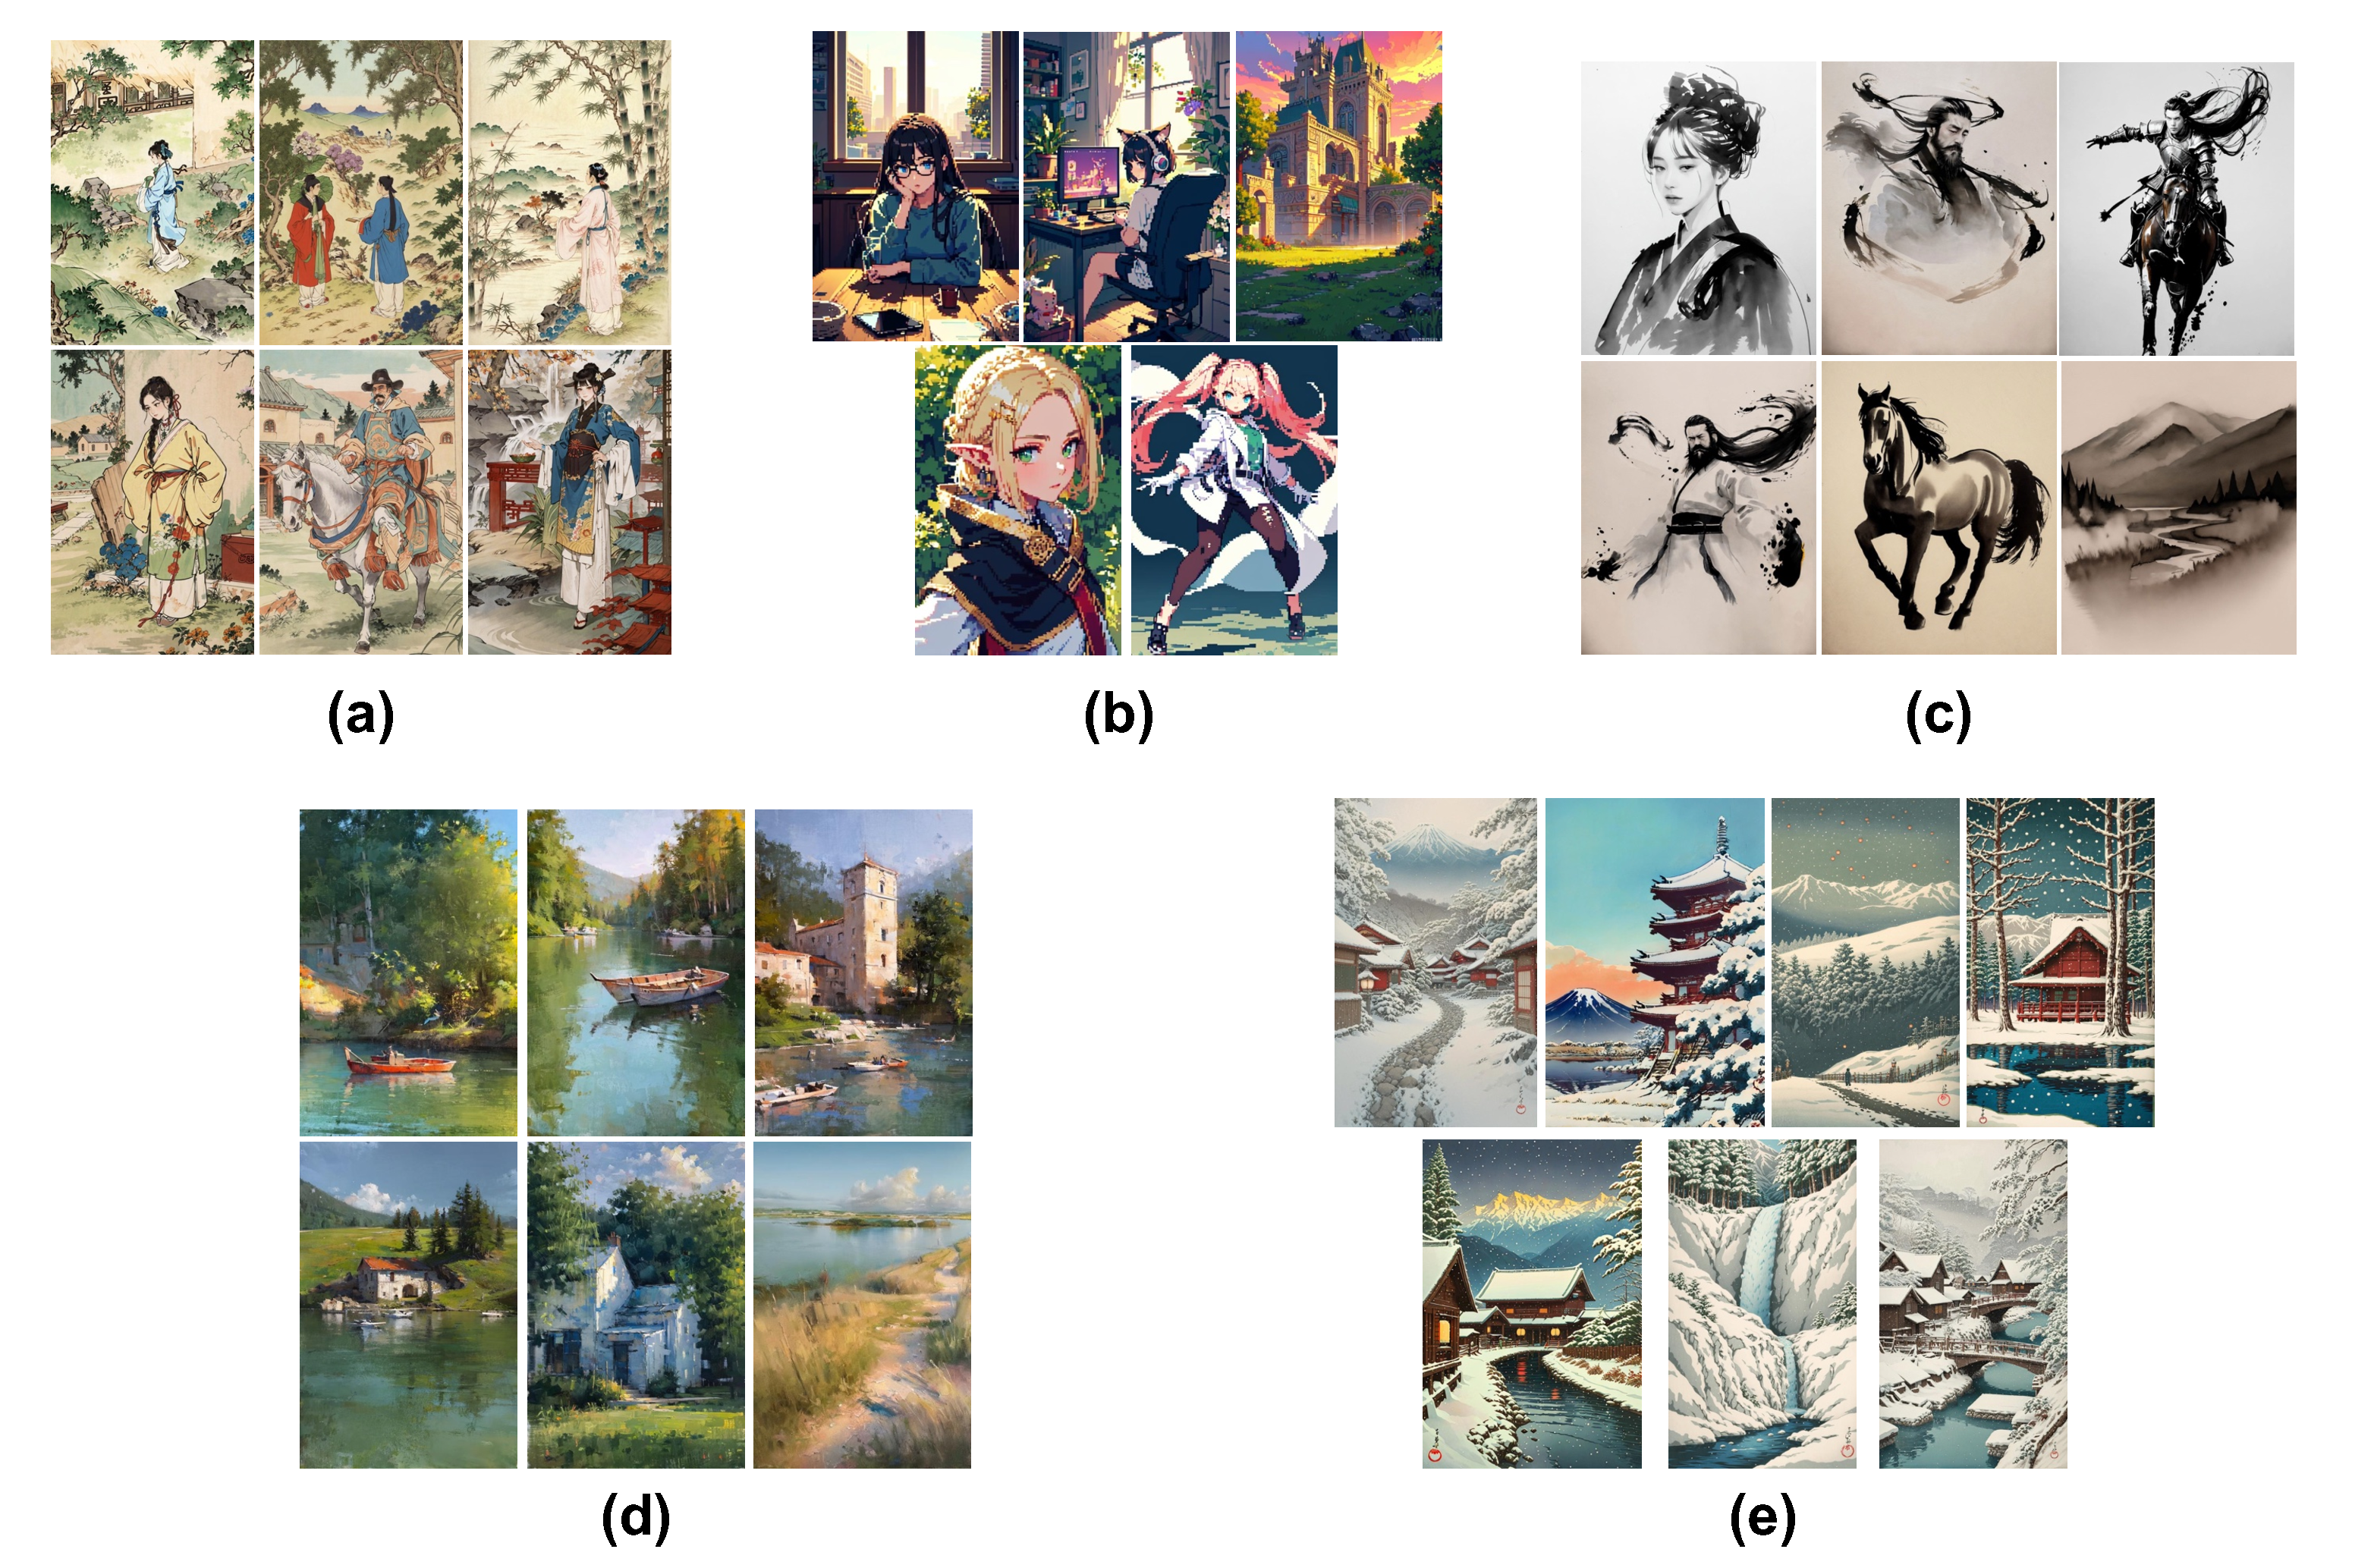
\includegraphics[width=0.85\linewidth]{figures/supp/multi_reference.pdf}
    \vspace{-1.2em}
    \captionof{figure}{Multiple references in the testset} 
    \label{fig:supp_multi_ref}
    \vspace{0.3em}


    \centering
    % \vspace{-0.5em}
    \captionof{table}{Text prompts used in the testset for image generation}
    \label{tab:supp_text_prompt_img}
    \vspace{-2.4em}
    \renewcommand{\arraystretch}{1.3}
    %\resizebox{0.99\linewidth}{!}{%
    \small
    \vspace{1.5em}
    \begin{tabular}{>{\centering\arraybackslash}p{5.5cm}>{\centering\arraybackslash}p{1.9cm}|>{\centering\arraybackslash}p{6.3cm}>{\centering\arraybackslash}p{1.9cm}} 
        %\toprule
        \hline
        Prompt & Meta Category & Prompt & Meta Category \\
        \hline
        %
        A man playing the guitar on a city street. & Human & A flock of birds flying gracefully in the sky. &  Animal \\
        %
        A woman reading a book in a park. & Human & A colorful butterfly resting on a flower. &  Animal \\
        %
        A couple dancing gracefully together. & Human & A bear fishing in a river. &  Animal \\
        %
        A person sitting on a bench, feeding birds. & Human & A dog running in front of a house. &  Animal \\
        %
        A person jogging along a scenic trail. & Human & A rabbit nibbling on a carrot. &  Animal \\
        %
        A bouquet of flowers in a vase. & Object & A cobblestone street lined with shops and cafes. &  Landscape \\
        %
        A telescope pointed at the stars. & Object & A modern cityscape with towering skyscrapers. &  Landscape \\
        %
        A rowboat docked on a peaceful lake. & Object & A winding path through a tranquil garden. &  Landscape \\
        %
        A lighthouse standing tall on a rocky coast. & Object & An ancient temple surrounded by lush vegetation. &  Landscape \\
        %
        A rustic windmill in a field. & Object & A serene mountain landscape with a river flowing through it. &  Landscape \\
        \hline
    \end{tabular}
    %}

    %%%%%%%%%%%%%%%%%%%%%%%%%
    \vspace{1.5em}
    \centering
    \captionof{table}{Text prompts used in the testset for video generation}
    \label{tab:supp_text_prompt_vid}
    \vspace{-1em}
    \begin{tabular}{>{\centering\arraybackslash}p{5.5cm}>{\centering\arraybackslash}p{1.9cm}|>{\centering\arraybackslash}p{6.3cm}>{\centering\arraybackslash}p{1.9cm}} 
        %\toprule
        \hline
        Prompt & Meta Category & Prompt & Meta Category \\
        \hline
        %
        A street performer playing the guitar. & Human & A bear catching fish in a river. &  Animal \\
        %
        A chef preparing meals in kitchen. & Human & A knight riding a horse through a field. &  Animal \\
        %
        A student walking to school with backpack. & Human & A wolf walking stealthily through the forest. &  Animal \\
        %
        A campfire surrounded by tents. & Object & A river flowing gently under a bridge. &  Landscape \\
        %
        A hot air balloon floating in the sky. & Object & A field of sunflowers on a sunny day. &  Landscape \\
        %
        A rocketship heading towards the moon. & Object & A wooden sailboat docked in a harbor. &  Landscape \\
        \hline
    \end{tabular}
    %}
\end{figure*}


\begin{table*}[!h]
    \centering
    \caption{Style references in the testset and corresponding style descriptions generated from GPT-4v\cite{openai2023gpt4v}.}
    \label{tab:supp_style_ref}
    \vspace{-1em}
    \renewcommand{\arraystretch}{1.1}
    %\resizebox{0.99\linewidth}{!}{%
    \small
    \begin{tabular}{>{\centering\arraybackslash}m{2.3cm}m{5.5cm}|>{\centering\arraybackslash}m{2.3cm}m{5.5cm}} 
        %\toprule
        \hline
        Style Reference & Style Descriptions & Style Reference & Style Descriptions \\
        \hline
        %
        \vspace{0.2cm}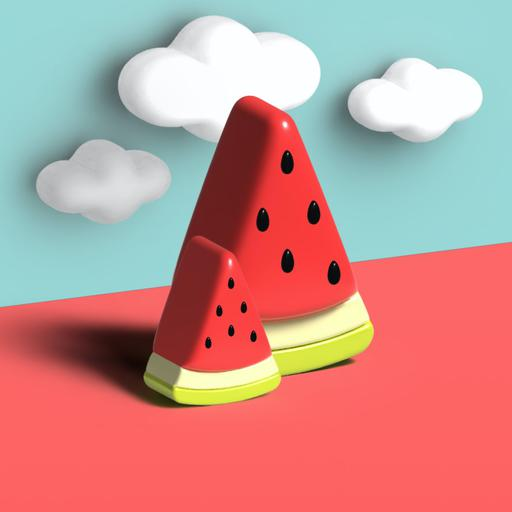
\includegraphics[width=2.3cm,height=1.7cm,keepaspectratio]{figures/style_figs/3d_1.jpg}
        & 3D Digital Art, {{\color{blue}{\{prompt\}}}}, whimsical and modern, smooth and polished surfaces, bold and contrasting colors, soft shading and lighting, surreal representation. 
        & \vspace{0.2cm}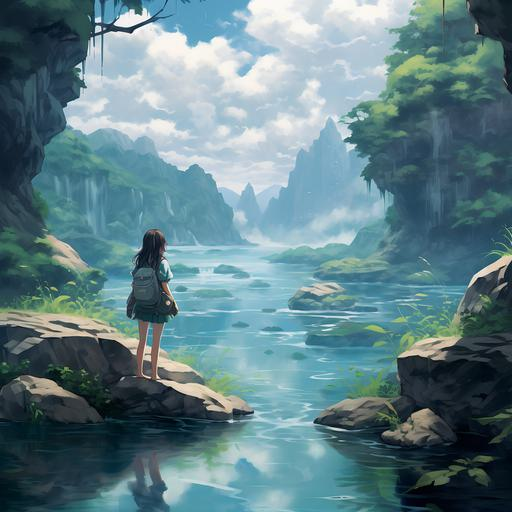
\includegraphics[width=2.3cm,height=1.7cm,keepaspectratio]{figures/style_figs/anime_1.jpg}
        & Digital Painting, {\color{blue}{\{prompt\}}}, detailed rendering, vibrant color palette, smooth gradients, realistic light and reflection, immersive natural landscape scene. \\
        %
        \vspace{0.2cm}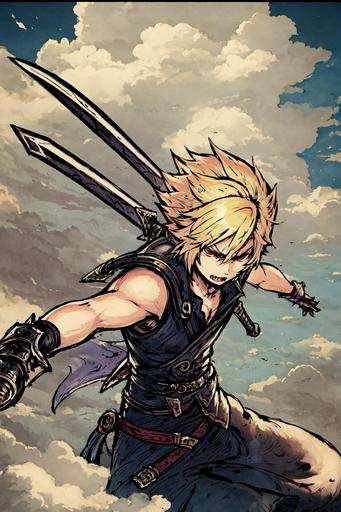
\includegraphics[width=2.3cm,height=1.7cm,keepaspectratio]{figures/style_figs/anime_2.jpg}
        & Manga-inspired digital art, {\color{blue}{\{prompt\}}}, dynamic composition, exaggerated proportions, sharp lines, cel-shading, high-contrast colors with a focus on sepia tones and blues. 
        & \vspace{0.2cm}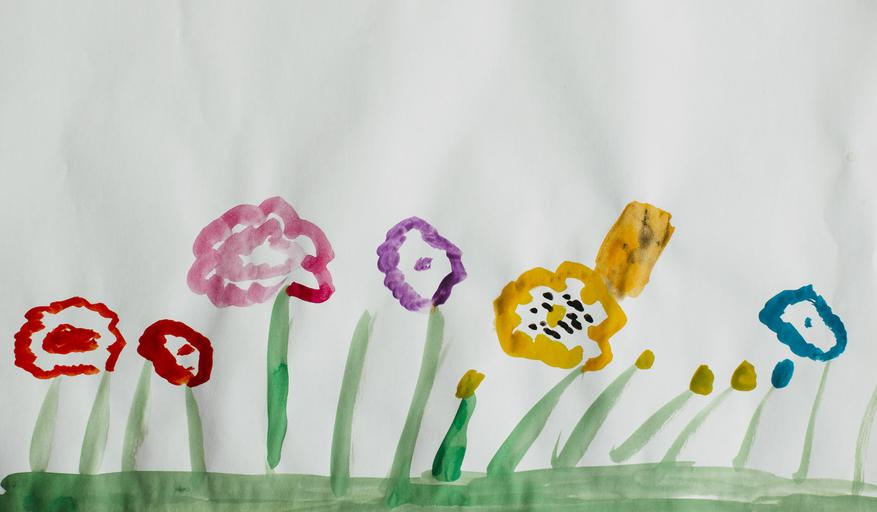
\includegraphics[width=2.3cm,height=1.7cm,keepaspectratio]{figures/style_figs/craft_1.jpg}
        & Childlike watercolor, {\color{blue}{\{prompt\}}}, simple brush strokes, primary and secondary colors, bold outlines, flat washes, playful, spontaneous, and expressive. \\
        %
        \vspace{0.2cm}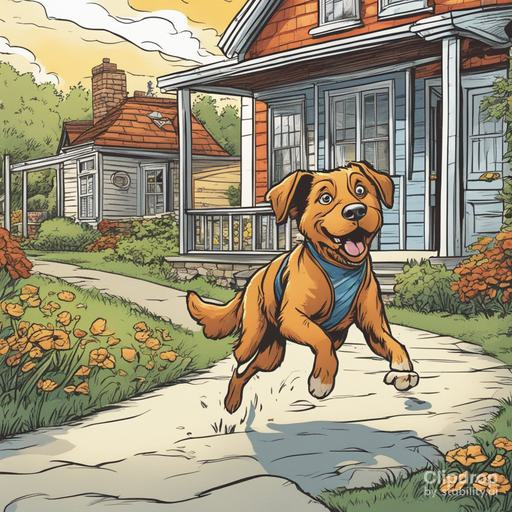
\includegraphics[width=2.3cm,height=1.7cm,keepaspectratio]{figures/style_figs/digital_art_1.jpg}
        & Comic book illustration, {\color{blue}{\{prompt\}}}, digital medium, clean inking, cell shading, saturated colors with a natural palette, and a detailed, textured background. 
        & \vspace{0.2cm}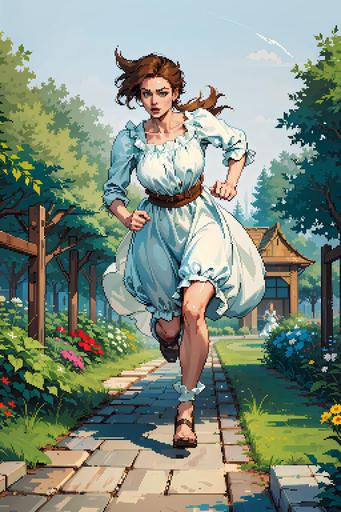
\includegraphics[width=2.3cm,height=1.7cm,keepaspectratio]{figures/style_figs/digital_art_2.jpg}
        & Pixel art illustration, {\color{blue}{\{prompt\}}}, digital medium, detailed sprite work, vibrant color palette, smooth shading, and a nostalgic, retro video game aesthetic. \\
        %
        \vspace{0.2cm}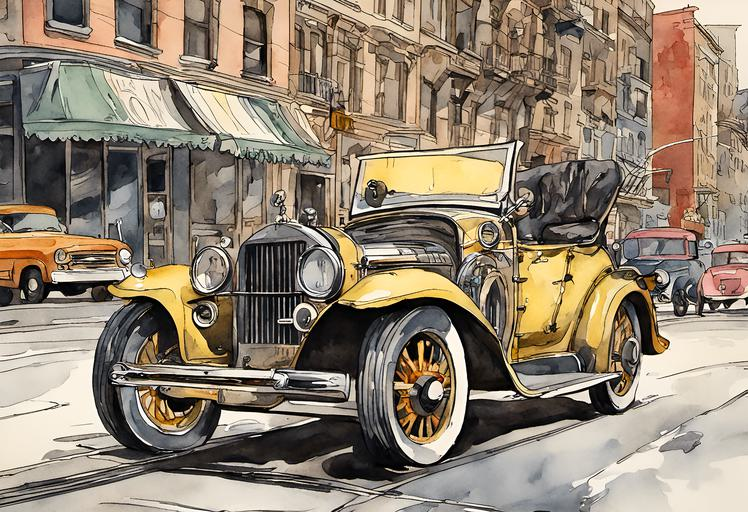
\includegraphics[width=2.3cm,height=1.7cm,keepaspectratio]{figures/style_figs/digital_art_3.jpg}
        & Ink and watercolor on paper, {\color{blue}{\{prompt\}}}, urban sketching style, detailed line work, washed colors, realistic shading, and a vintage feel.
        & \vspace{0.2cm}
\includegraphics[width=2.3cm,height=1.7cm,keepaspectratio]{figures/style_figs/icon_1.jpg}
        & Flat Vector Illustration, {\color{blue}{\{prompt\}}}, simplified shapes, uniform color fills, minimal shading, absence of texture, clean and modern aesthetic. \\
        %
        \vspace{0.2cm}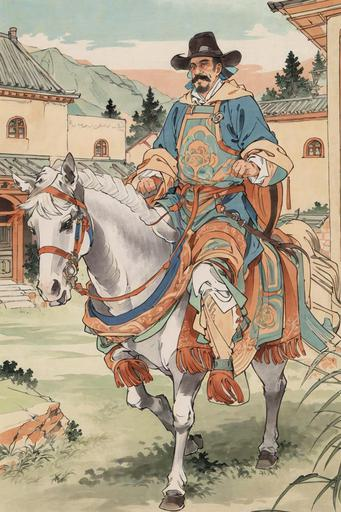
\includegraphics[width=2.3cm,height=1.7cm,keepaspectratio]{figures/style_figs/illstration_1.jpg}
        & Watercolor and ink illustration, {\color{blue}{\{prompt\}}}, traditional comic style, muted earthy color palette, detailed with a sense of movement, soft shading, and a historic ambiance. 
        & \vspace{0.2cm}
\includegraphics[width=2.3cm,height=1.7cm,keepaspectratio]{figures/style_figs/illustration_2.jpg}
        & Low Poly Digital Art, {\color{blue}{\{prompt\}}}, geometric shapes, vibrant colors, flat texture, sharp edges, gradient shading, modern graphic style. \\
        %
        \vspace{0.2cm}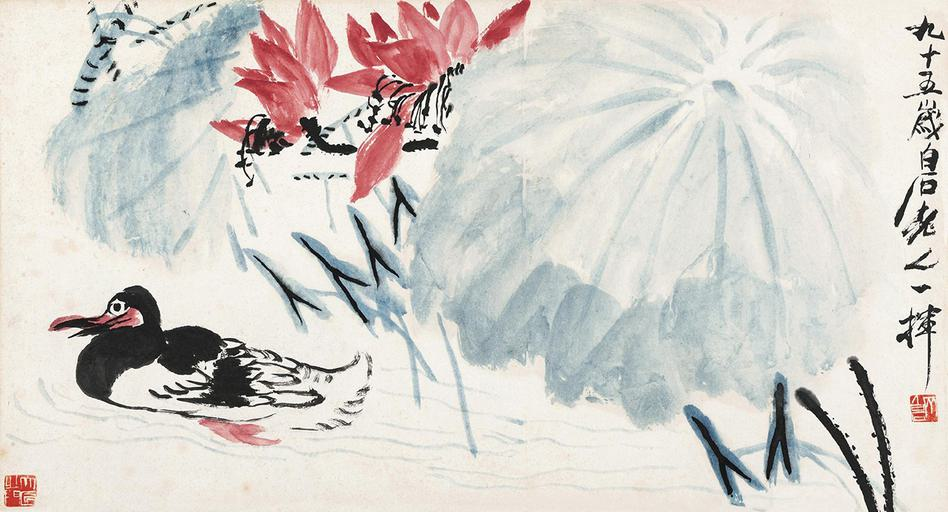
\includegraphics[width=2.3cm,height=1.7cm,keepaspectratio]{figures/style_figs/ink_1.jpg}
        & Chinese ink wash painting, {\color{blue}{\{prompt\}}}, minimalistic color use, calligraphic brushwork, emphasis on flow and balance, with poetic inscription.
        & \vspace{0.2cm}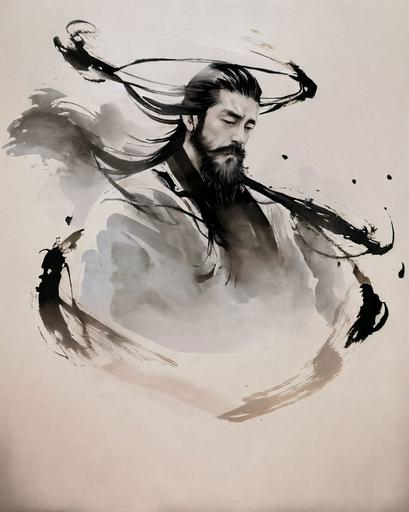
\includegraphics[width=2.3cm,height=1.7cm,keepaspectratio]{figures/style_figs/ink_2.jpg}
        & Chinese Ink Wash Painting, {\color{blue}{\{prompt\}}}, monochromatic palette, dynamic brushstrokes, calligraphic lines, with a focus on negative space and movement. \\
        %
        \vspace{0.2cm}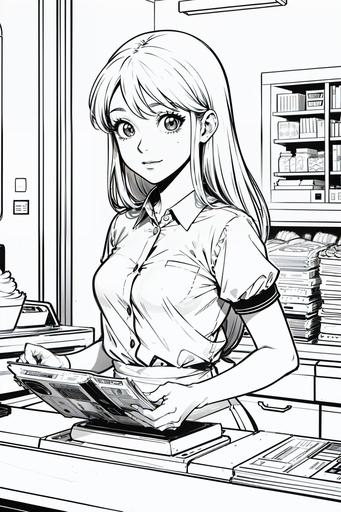
\includegraphics[width=2.3cm,height=1.7cm,keepaspectratio]{figures/style_figs/line_1.jpg}
        & Manga Style, {\color{blue}{\{prompt\}}}, black and white digital inking, high contrast, detailed line work, cross-hatching for shadows, clean, no color.
        & \vspace{0.2cm}
\includegraphics[width=2.3cm,height=1.7cm,keepaspectratio]{figures/style_figs/line_2.jpg}
        & Line Drawing, {\color{blue}{\{prompt\}}}, simple and clean lines, monochrome palette, smooth texture, minimalist and cartoonish representation . \\
        %
        \vspace{0.2cm}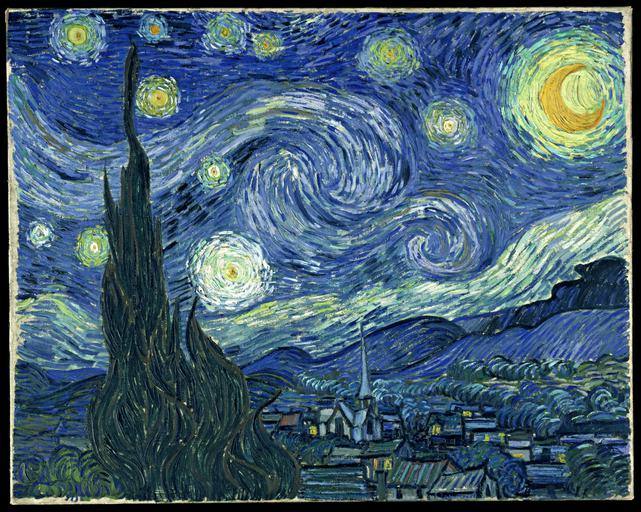
\includegraphics[width=2.3cm,height=1.7cm,keepaspectratio]{figures/style_figs/oil_paint_1.jpg}
        & Van Gogh's "Starry Night" style, {\color{blue}{\{prompt\}}}, with expressive, swirling brushstrokes, rich blue and yellow palette, and bold, impasto texture. 
        & \vspace{0.2cm}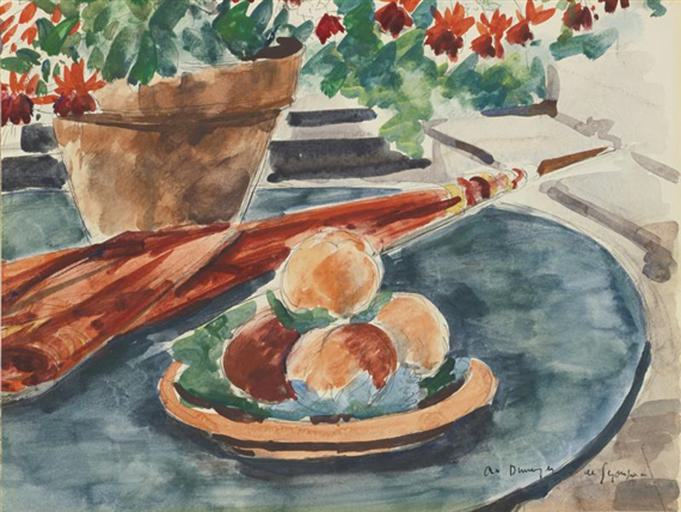
\includegraphics[width=2.3cm,height=1.7cm,keepaspectratio]{figures/style_figs/oil_paint_2.jpg}
        & Watercolor Painting, {\color{blue}{\{prompt\}}}, fluid brushstrokes, transparent washes, color blending, visible paper texture, impressionistic style. \\
        %
        \vspace{0.2cm}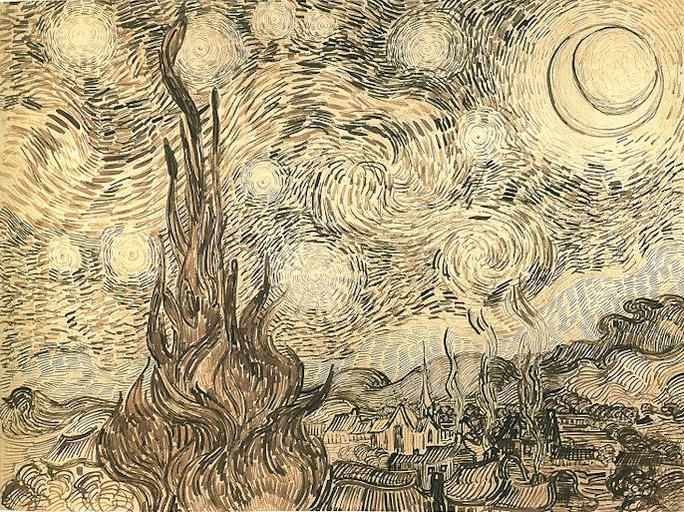
\includegraphics[width=2.3cm,height=1.7cm,keepaspectratio]{figures/style_figs/oil_paint_3.jpg}
        & Van Gogh-inspired pen sketch, {\color{blue}{\{prompt\}}}, dynamic and swirling line work, monochromatic sepia tones, textured with a sense of movement and energy. 
        & \vspace{0.2cm}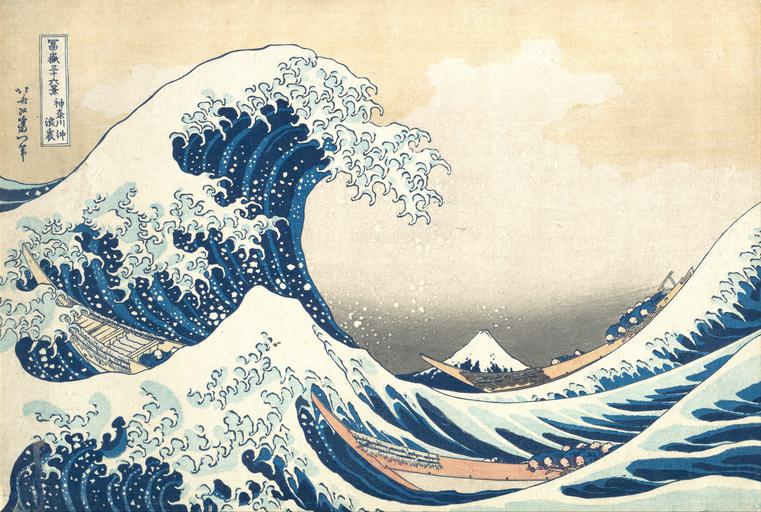
\includegraphics[width=2.3cm,height=1.7cm,keepaspectratio]{figures/style_figs/ukiyoe.jpg}
        & Ukiyo-e Woodblock Print, {\color{blue}{\{prompt\}}}, gradation, limited color palette, flat areas of color, expressive line work, stylized wave forms, traditional Japanese art. \\
        %
        \vspace{0.2cm}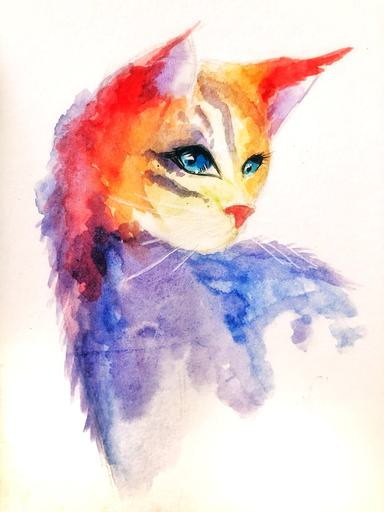
\includegraphics[width=2.3cm,height=1.7cm,keepaspectratio]{figures/style_figs/watercolor_1.jpg}
        & Watercolor Painting, {\color{blue}{\{prompt\}}}, fluid washes of color, wet-on-wet technique, vibrant hues, soft texture, impressionistic portrayal.
        & \vspace{0.2cm}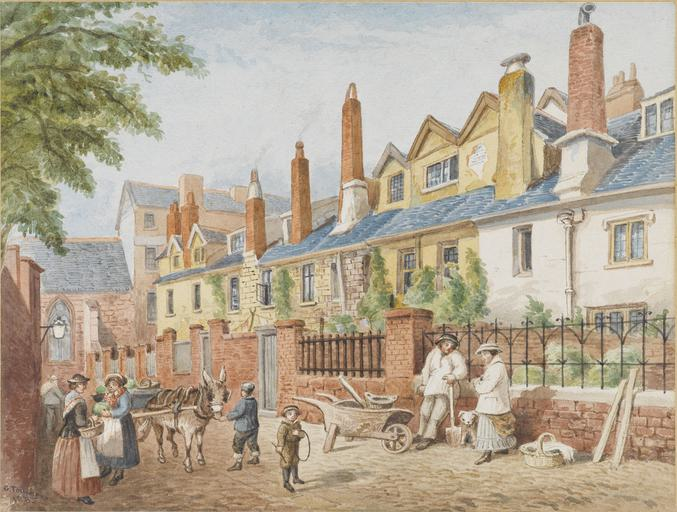
\includegraphics[width=2.3cm,height=1.7cm,keepaspectratio]{figures/style_figs/watercolor_2.jpg}
        & Victorian watercolor, {\color{blue}{\{prompt\}}}, fine detail, soft pastel hues, gentle lighting, clear texture, with a quaint, realistic portrayal of everyday life. \\
        \hline
    \end{tabular}
    %}
\end{table*}

%
\begin{figure*}[p]
    \centering
    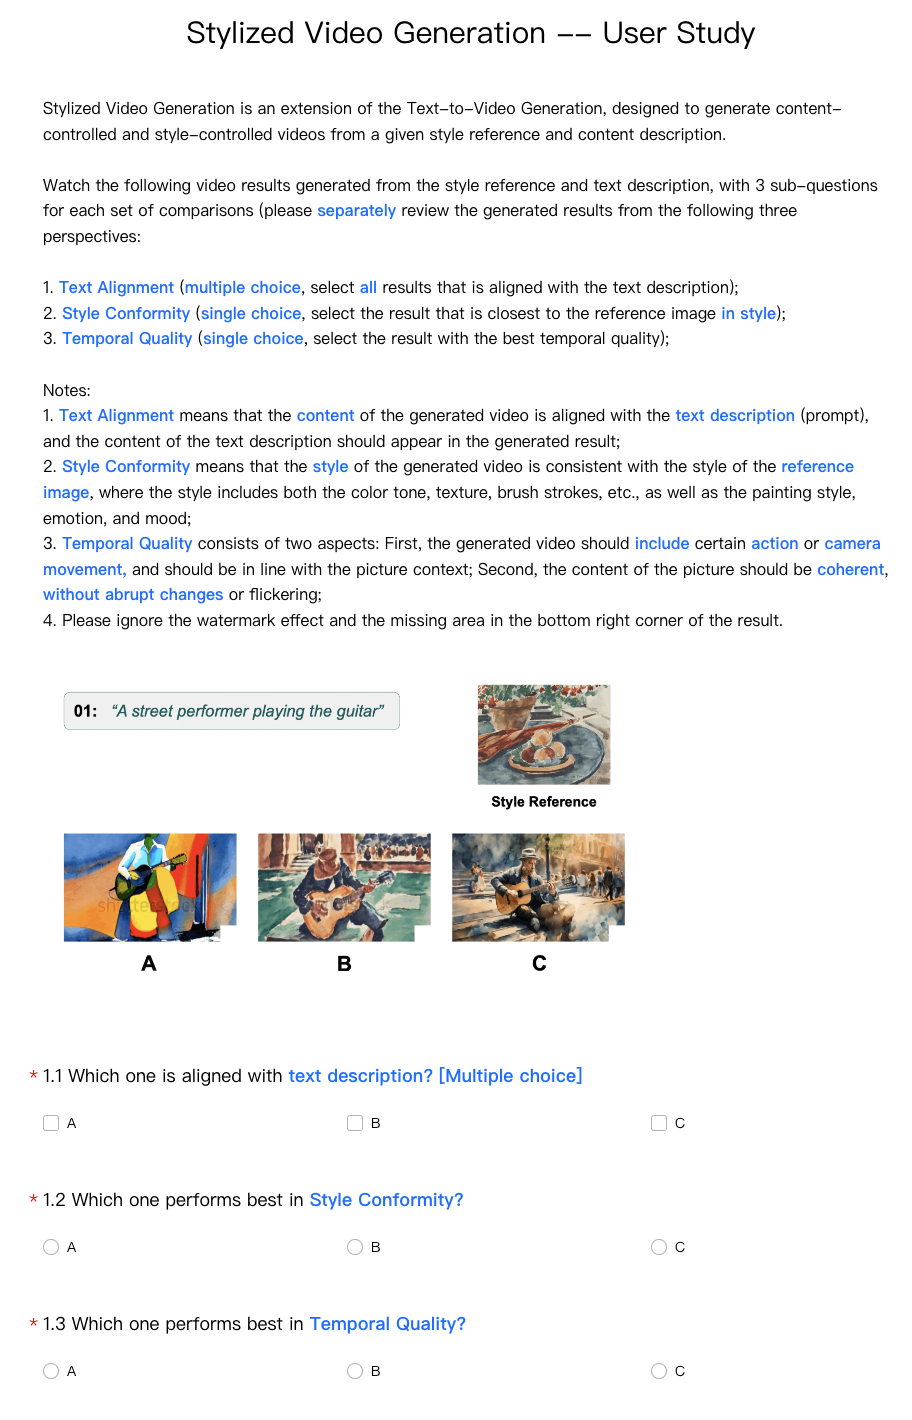
\includegraphics[width=0.72\linewidth]{figures/supp/user_study_2.png}
    \caption{User Preference Study Interface} 
    \label{fig:supp_user_study}
\end{figure*}

%
% For text alignment, participants were instructed to select all results that aligned with the text description. For style conformity, they were asked to choose the result that most closely resembled the reference image in style. For temporal quality, participants were instructed to select the result with the best temporal quality, which included both obvious actions and temporal consistency. 
%

\section{Evaluation Details}
\label{sec:supp_eval}
\subsection{Evaluation Metrics}

We employ CLIP-based similarity scores to evaluate text alignment and style conformity, as is commonly done by existing methods. Additionally, we include two metrics to measure the temporal consistency of generated videos, i.e., \textit{CLIP-Temp} and \textit{Warping Error}. A detailed calculation process for each metric is presented below.

\paragraph{CLIP-Text} We utilize the pretrained CLIP-ViT-H-14-laion2B-s32B-b79K\footnote{\url{https://huggingface.co/laion/CLIP-ViT-H-14-laion2B-s32B-b79K}} as a feature extractor(also for \textit{CLIP-Style} and \textit{CLIP-Temp}), which is trained on LAION-2B and demonstrates enhanced performance across various datasets. We extract the frame-wise image embeddings from the generated results and text embeddings from the input content prompts, then compute their average cosine similarity. The overall \textit{CLIP-Text} is calculated as:

\begin{equation}
    S_{text} = \frac{1}{M}\sum_{i = 1}^{M}(\frac{1}{T}\sum_{t=1}^{T}\frac{emb(x_t^i) \cdot emb(p^i)}{\lVert emb(x_t^i) \rVert \cdot \lVert emb(p^i) \rVert})
\end{equation}
where $M$ represents the total number of testing videos and $T$ represents the total number of frames in each video($T = 1$ for image generation), $emb(x_t^i)$ and $emb(p^i)$ indicate the CLIP embedding of the $t$-th frame of the $i$-th video $x_t^i$ and the corresponding prompt $p^i$, respectively.

\paragraph{CLIP-Style} Similarly, we extract the frame-wise image embeddings $emb(x_t^i)$ from the generated results and image embeddings $s^i$ from the input style reference. The overall \textit{CLIP-Text} is calculated as:

\begin{equation}
    S_{style} = \frac{1}{M}\sum_{i = 1}^{M}(\frac{1}{T}\sum_{t=1}^{T}\frac{emb(x_t^i) \cdot emb(s^i)}{\lVert emb(x_t^i) \rVert \cdot \lVert emb(s^i) \rVert})
\end{equation}

\paragraph{CLIP-Temp} Considering the semantic consistency between every two frames, we extract the frame-wise CLIP image embeddings and compute the cosine similarity between each of the two frames, as follows:

\begin{equation}
    S_{temp} = \frac{1}{M}\sum_{i = 1}^{M}(\frac{1}{T-1}\sum_{t=1}^{T - 1}\frac{emb(x_t^i) \cdot emb(x_{t + 1}^i)}{\lVert emb(x_t^i) \rVert \cdot \lVert emb(x_{t + 1}^i) \rVert})
\end{equation}

\paragraph{Warping Error} For the warping error, we first obtain the optical flow between each two frames using RAFT-small\cite{teed2020raft}, a pre-trained optical flow estimation network. Subsequently, we compute the pixel-wise differences between the warped image and the predicted image, as follows:

\begin{equation}
    W_{error} = \frac{1}{M}\sum_{i = 1}^{M}(\frac{1}{T-1}\sum_{t=1}^{T - 1} \lVert x_t^i - warp(x_{t + 1}^i, flow(x_{t + 1}^i, x_{t}^i))\rVert)
\end{equation}
where $warp(x_{t + 1}^i, flow(x_{t + 1}^i, x_{t}^i))$ represents the warped frame of $x_{t + 1}^i$ using the optical flow between frame $x_{t + 1}^i$ and frame $x_{t}^i$.


\subsection{User Study}

In this subsection, we provide a detailed introduction about our user study. We randomly selected 15 single-reference style-text pairs to compare the generated results among VideoCrafter~\cite{chen2023videocrafter}, Gen-2~\cite{Gen-2}, and our proposed method. Given that videocomposer~\cite{wang2024videocomposer} directly replicates the style reference and is minimally influenced by the prompt in most cases, we excluded it from the comparison in the user study. Additionally, we randomly chose 10 multi-reference style-text pairs for the comparison between AnimateDiff~\cite{guo2023animatediff} (multiple style-specific models) and our method (a generic model). To ensure a blind comparison, we randomized the order of options for each question and masked the possible model watermark in the lower right corner.

The designed user preference interface is illustrated in Figure~\ref{fig:supp_user_study}. We invited 15 users of normal eyesight to evaluate the generated results in three aspects: text alignment, style conformity, and temporal quality.  The instructions and questions are provided as below.
%
% For text alignment, participants were instructed to select all results that aligned with the text description. For style conformity, they were asked to choose the result that most closely resembled the reference image in style. For temporal quality, participants were instructed to select the result with the best temporal quality, which included both obvious actions and temporal consistency. 
%
Consequently, a total of 1125 votes are collected.\vspace{0.6em}


\noindent\textbf{Instructions.}

\begin{itemize}[leftmargin=2.0em]
    \item \textbf{Task}: Watch the following video results generated from the style reference and text description, with 3 sub-questions for each set of comparisons (please \textbf{separately} review the generated results from the following three perspectives:

    \begin{itemize}[leftmargin=2.0em]
        \item \textbf{Text Alignment} (multiple choice, means that the content of the generated video is aligned with the text description(prompt), and the content of the text description should appear in the generated result);
        \item \textbf{Style Conformity} (single choice, means that the style of the generated video is consistent with the style of the reference image, where the style includes both the color tone, texture, brush strokes, etc., as well as the painting style, emotion, and mood);
        \item \textbf{Temporal Quality} (single choice, consists of two aspects: First, the generated video should include certain action or camera movement, and should be in line with the picture context; Second, the content of the picture should be coherent, without abrupt changes or flickering);
    \end{itemize}
    
    \item Please ignore the watermark effect and the missing area in the bottom right corner of the result.
    % \begin{itemize}
    %     \item Text Alignment means that the content of the generated video is aligned with the text description(prompt), and the content of the text description should appear in the generated result;
    %     \item Style Conformity means that the style of the generated video is consistent with the style of the reference image, where the style includes both the color tone, texture, brush strokes, etc., as well as the painting style, emotion, and mood;
    %     \item Temporal Quality consists of two aspects: First, the generated video should include certain action or camera movement, and should be in line with the picture context; Second, the content of the picture should be coherent, without abrupt changes or flickering;
    %     \item Please ignore the watermark effect and the missing area in the bottom right corner of the result.
    % \end{itemize}
\end{itemize}

% \vspace{0.6em}
\noindent\textbf{Questions.}

\begin{itemize}[leftmargin=2.0em]
    \item Which one is aligned with text description? \textbf{[Multiple choice]}
    \item Which performs best in Style Conformity? \textbf{[Single choice]}
    \item Which performs best in Temporal Quality? \textbf{[Single choice]}
\end{itemize}
 

%%%%%%%%%%%%%%%%%%%%%%%%%%%%%%%%%
\section{Extended Comparison}
\label{sec:supp_extend_comp}

\subsection{Multi-reference Stylized Image Generation}

\begin{figure*}[!h]
    \centering
    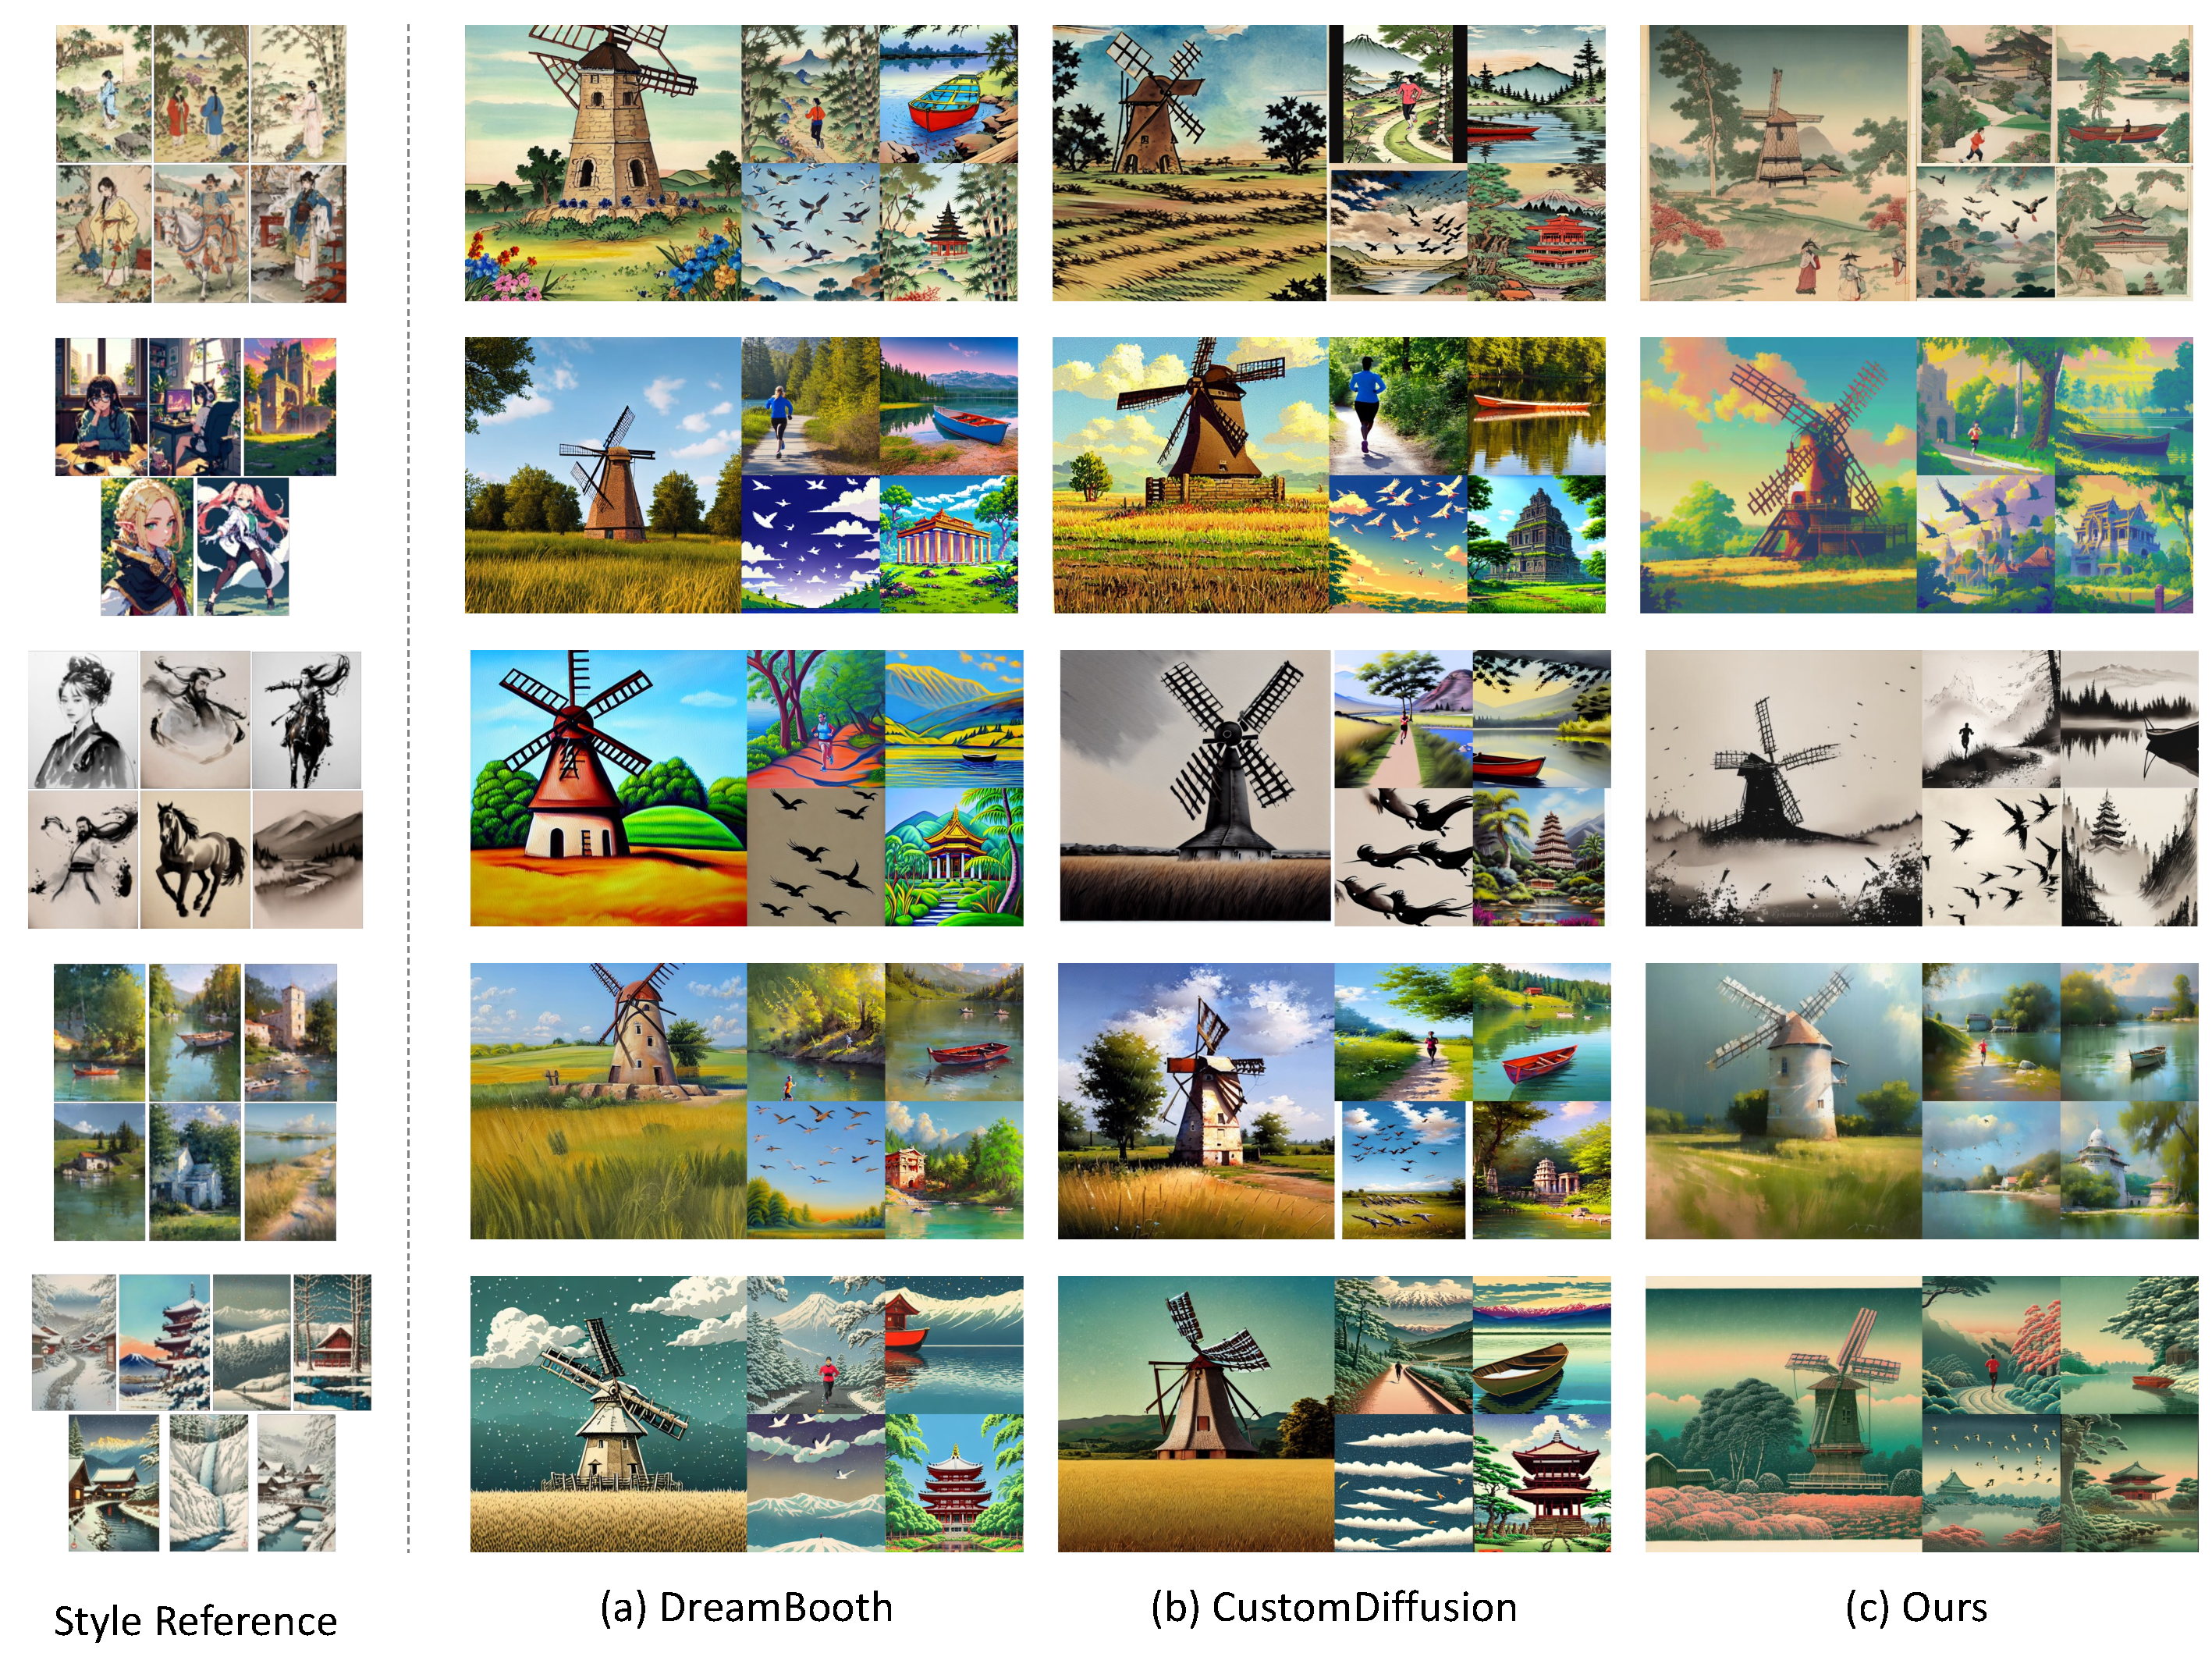
\includegraphics[width=0.9\linewidth]{figures/supp/result_comp_multi_ref.pdf}
    \vspace{-1.5em}
    \caption{Visual comparison on mulit-reference stylized T2I generation. Testing prompts: (i) \textit{A rustic windmill in a field.}; (ii) \textit{A person jogging along a scenic trail.}; (iii) \textit{A flock of birds flying gracefully in the sky.}; (iv) \textit{A rowboat docked on a peaceful lake.}; (v) \textit{An ancient temple surrounded by lush vegetation.}} 
    \label{fig:supp_comp_multi_ref}
\end{figure*}


We conduct comparisons of multi-reference stylized image generation with Dreambooth~\cite{dreambooth} and CustomDiffusion~\cite{customdiffusion}, both of which support generating images in specific styles by finetuning on the reference images. Figure~\ref{fig:supp_multi_ref} and Table~\ref{tab:supp_multi_ref} present the visual and quantitative results respectively, demonstrating that our method surpasses all competitors in terms of style conformity for multi-reference stylized generation. Although Dreambooth and CustomDiffusion exhibit competitive performance in certain cases, their stylized generation abilities tend to vary with different prompts, i.e., struggling to maintain consistent visual styles across arbitrary prompts. It is possibly because several images are insufficient to allow the model to disentangle the contents and styles, thus harming the generalization performance.
Besides, the requirement for finetuning during the testing process also undermines their flexibility. In contrast, our method efficiently generates high-quality stylized images that align with the prompts and conform the style of reference images without additional finetuning costs.


%
\begin{table}[!h]
\centering
\caption{Quantitative comparison on Multi-reference style-guided T2I generation. \textbf{Bold}: Best.}
\label{tab:supp_multi_ref}
\vspace{-1.0em}
%\setlength{\tabcolsep}{3.0pt}
% \renewcommand\arraystretch{1.5}
%\resizebox{\linewidth}{!}{
  \begin{tabular}{ccccc} % {@{}lc@{}}
    % \toprule
    %  \hline
    %  & \multicolumn{5}{|c}{\textbf{CLIP scores}} \\
    \hline
    Methods & Dreambooth & CustomDiffsion  & Ours \\
    \hline
    \texttt{Text} $\uparrow$ & 0.2868 & \textbf{0.2986} & 0.2924 \\
    \texttt{Style} $\uparrow$ & 0.4270 & 0.4441 & \textbf{0.5333} \\
    \hline
  \end{tabular}
% }
\end{table}


% \subsection{Comparison with AnimateDiff}
% \TODO{(11.23) 1. We have pretrained a good personalized T2I model, but it has degraded in performance of style and temporal. 2. Our performance is comparable with AnimateDiff + their good personalized model.}

\vspace{-1.0em}
\subsection{Comparison with StyleDrop}

\begin{figure*}[!t]
    \centering
    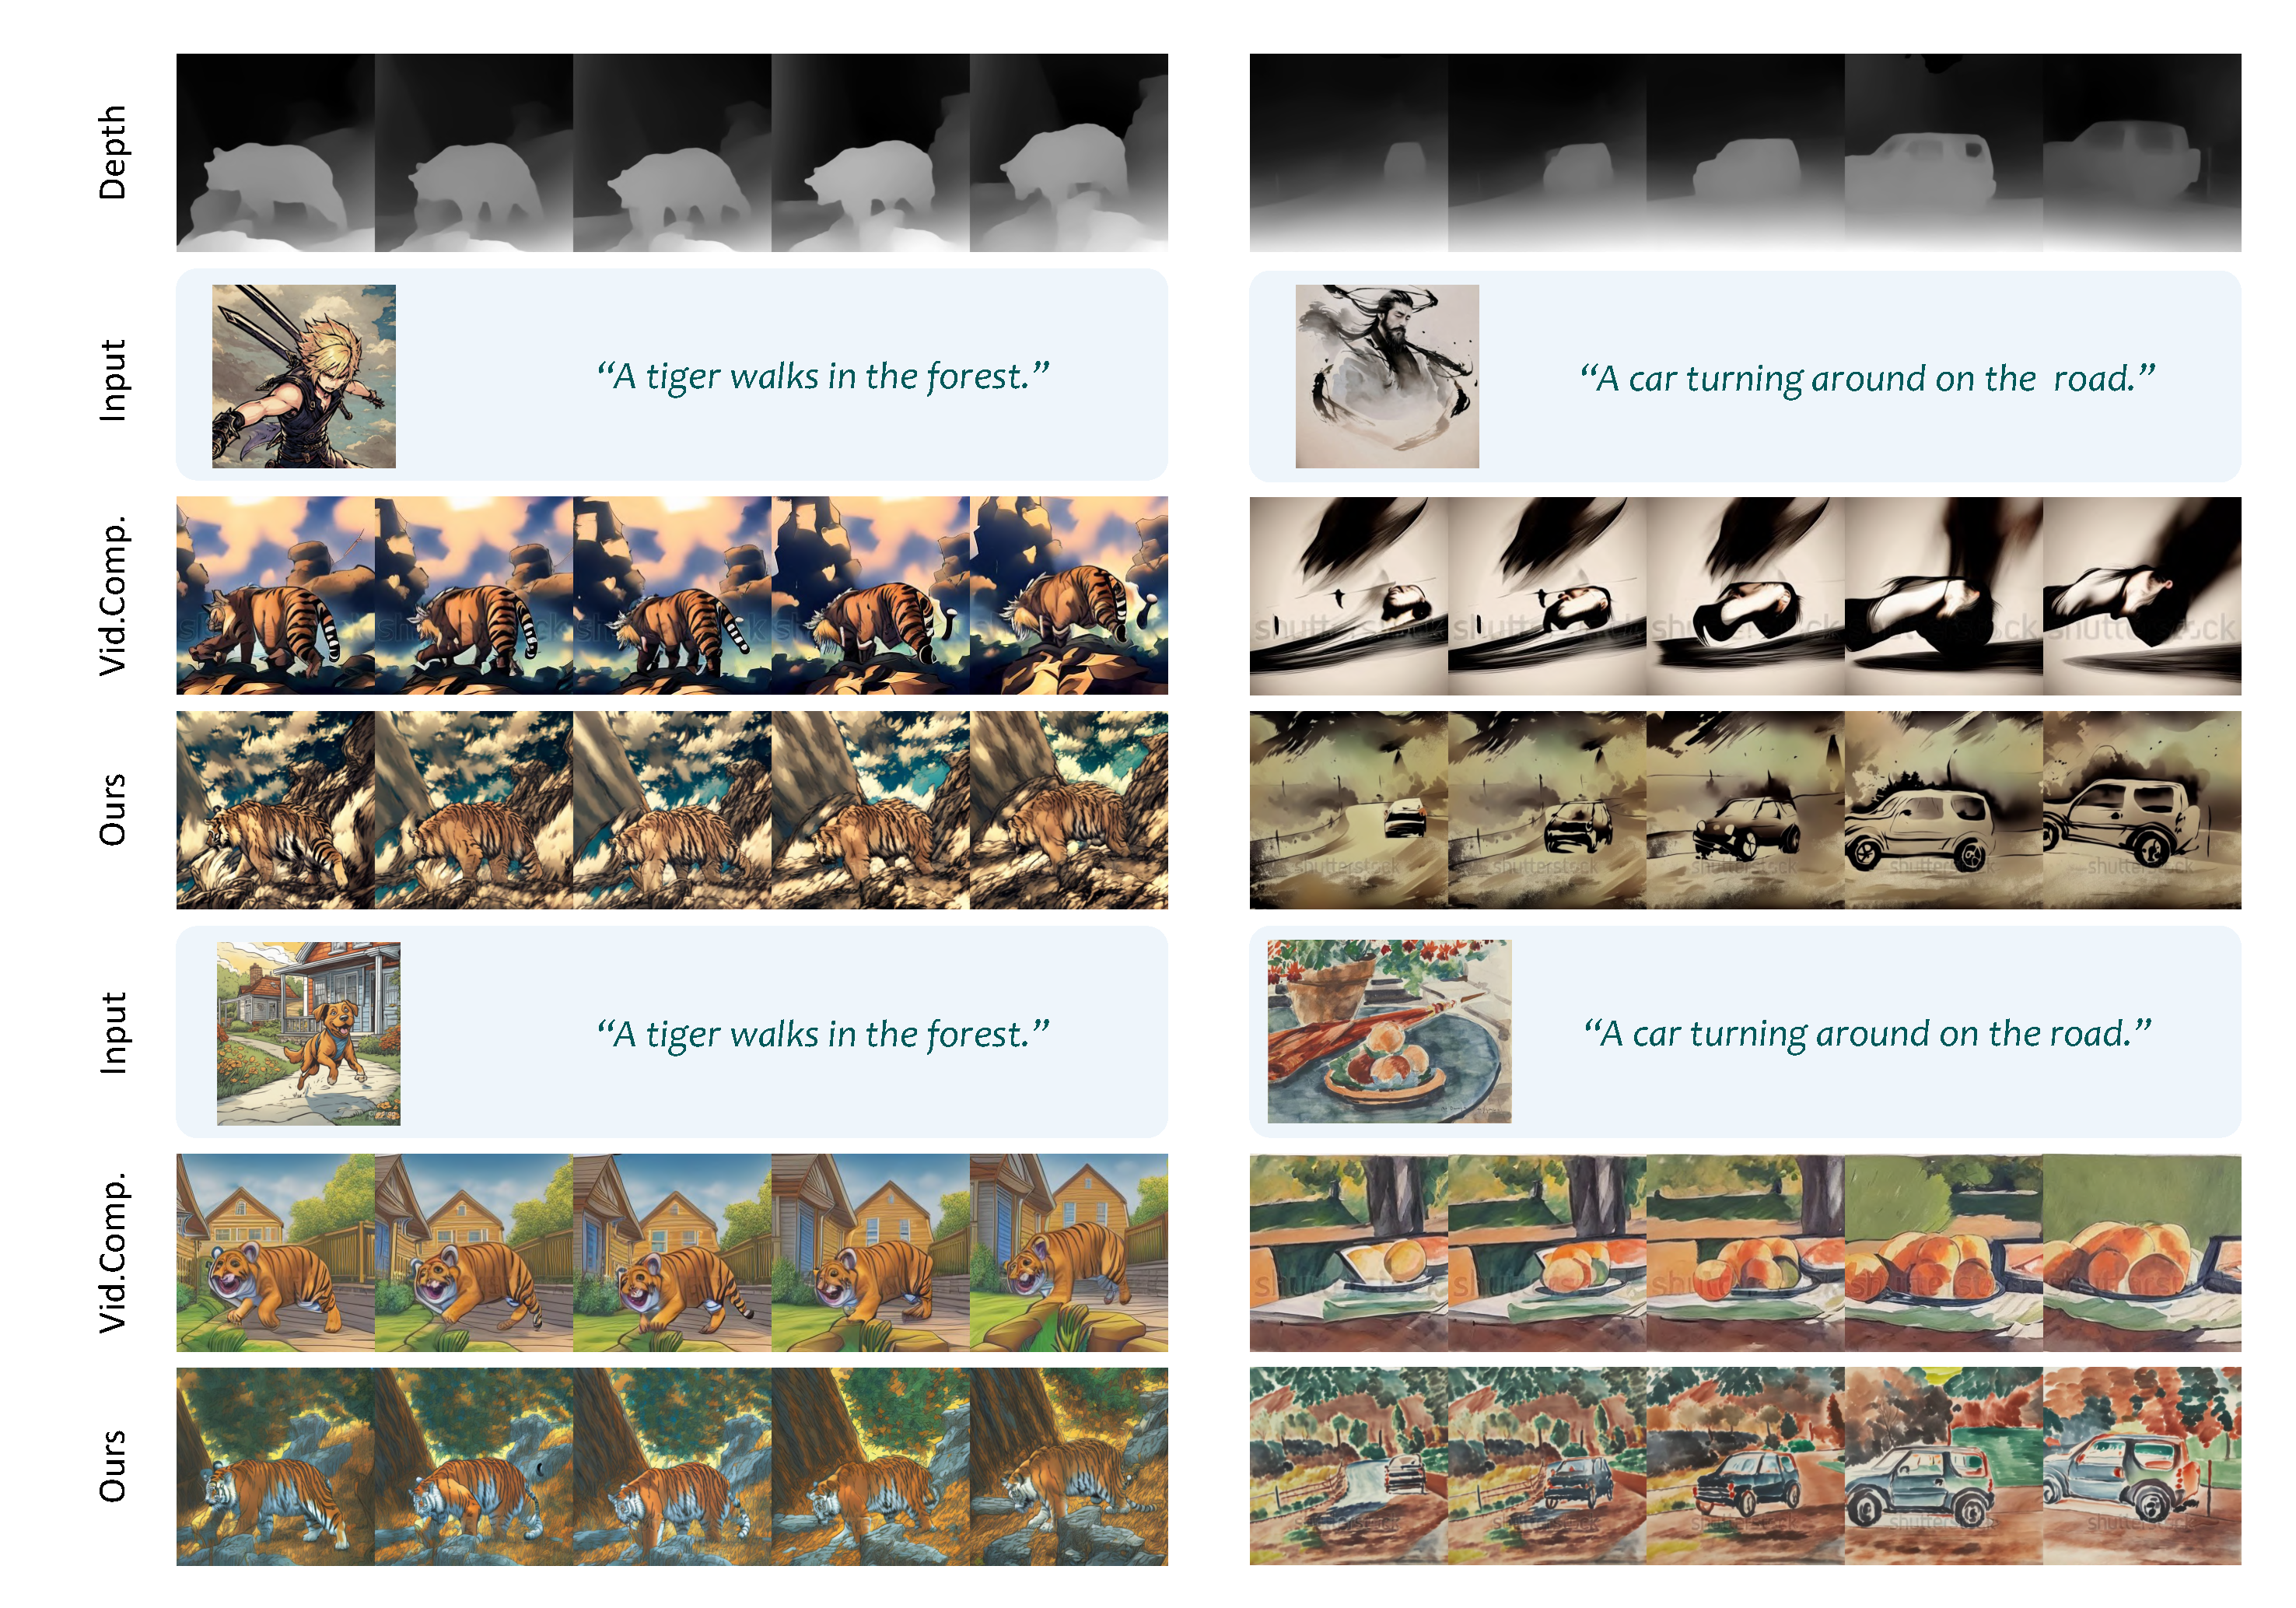
\includegraphics[width=\linewidth]{figures/supp/result_depth.pdf}
    \vspace{-2em}
    \caption{Visual comparison on stylized video generation with additional depth guidance. Vid.Comp.: VideoComposer} 
    \label{fig:supp_depth}
\end{figure*}


Here we present a supplementary comparison with StyleDrop\cite{sohn2023styledrop}. StyleDrop proposes a versatile method for synthesizing images that faithfully follow a specific style using a text-to-image model. Owing to the absence of an official StyleDrop implementation, we have excluded the comparison with StyleDrop from the main text. Instead, we include a comparison with an unofficial StyleDrop implementation\footnote{\url{https://github.com/aim-uofa/StyleDrop-PyTorch}} here. We train StyleDrop based on StableDiffusion 2.1 for 1000 steps with a batch size of 8 and a learning rate of $3 \times 10^{-4}$. The quantitative and qualitative results are presented in Table~\ref{tab:supp_comp_styledrop} and Figure~\ref{fig:supp_comp_styledrop} respectively. Results show that compared to StyleDrop, our proposed method more effectively captures the visual characteristics of a user-provided style and combines them with various prompts in a flexible manner.

\begin{figure}[!h]
    \centering
    \vspace{-0.8em}
    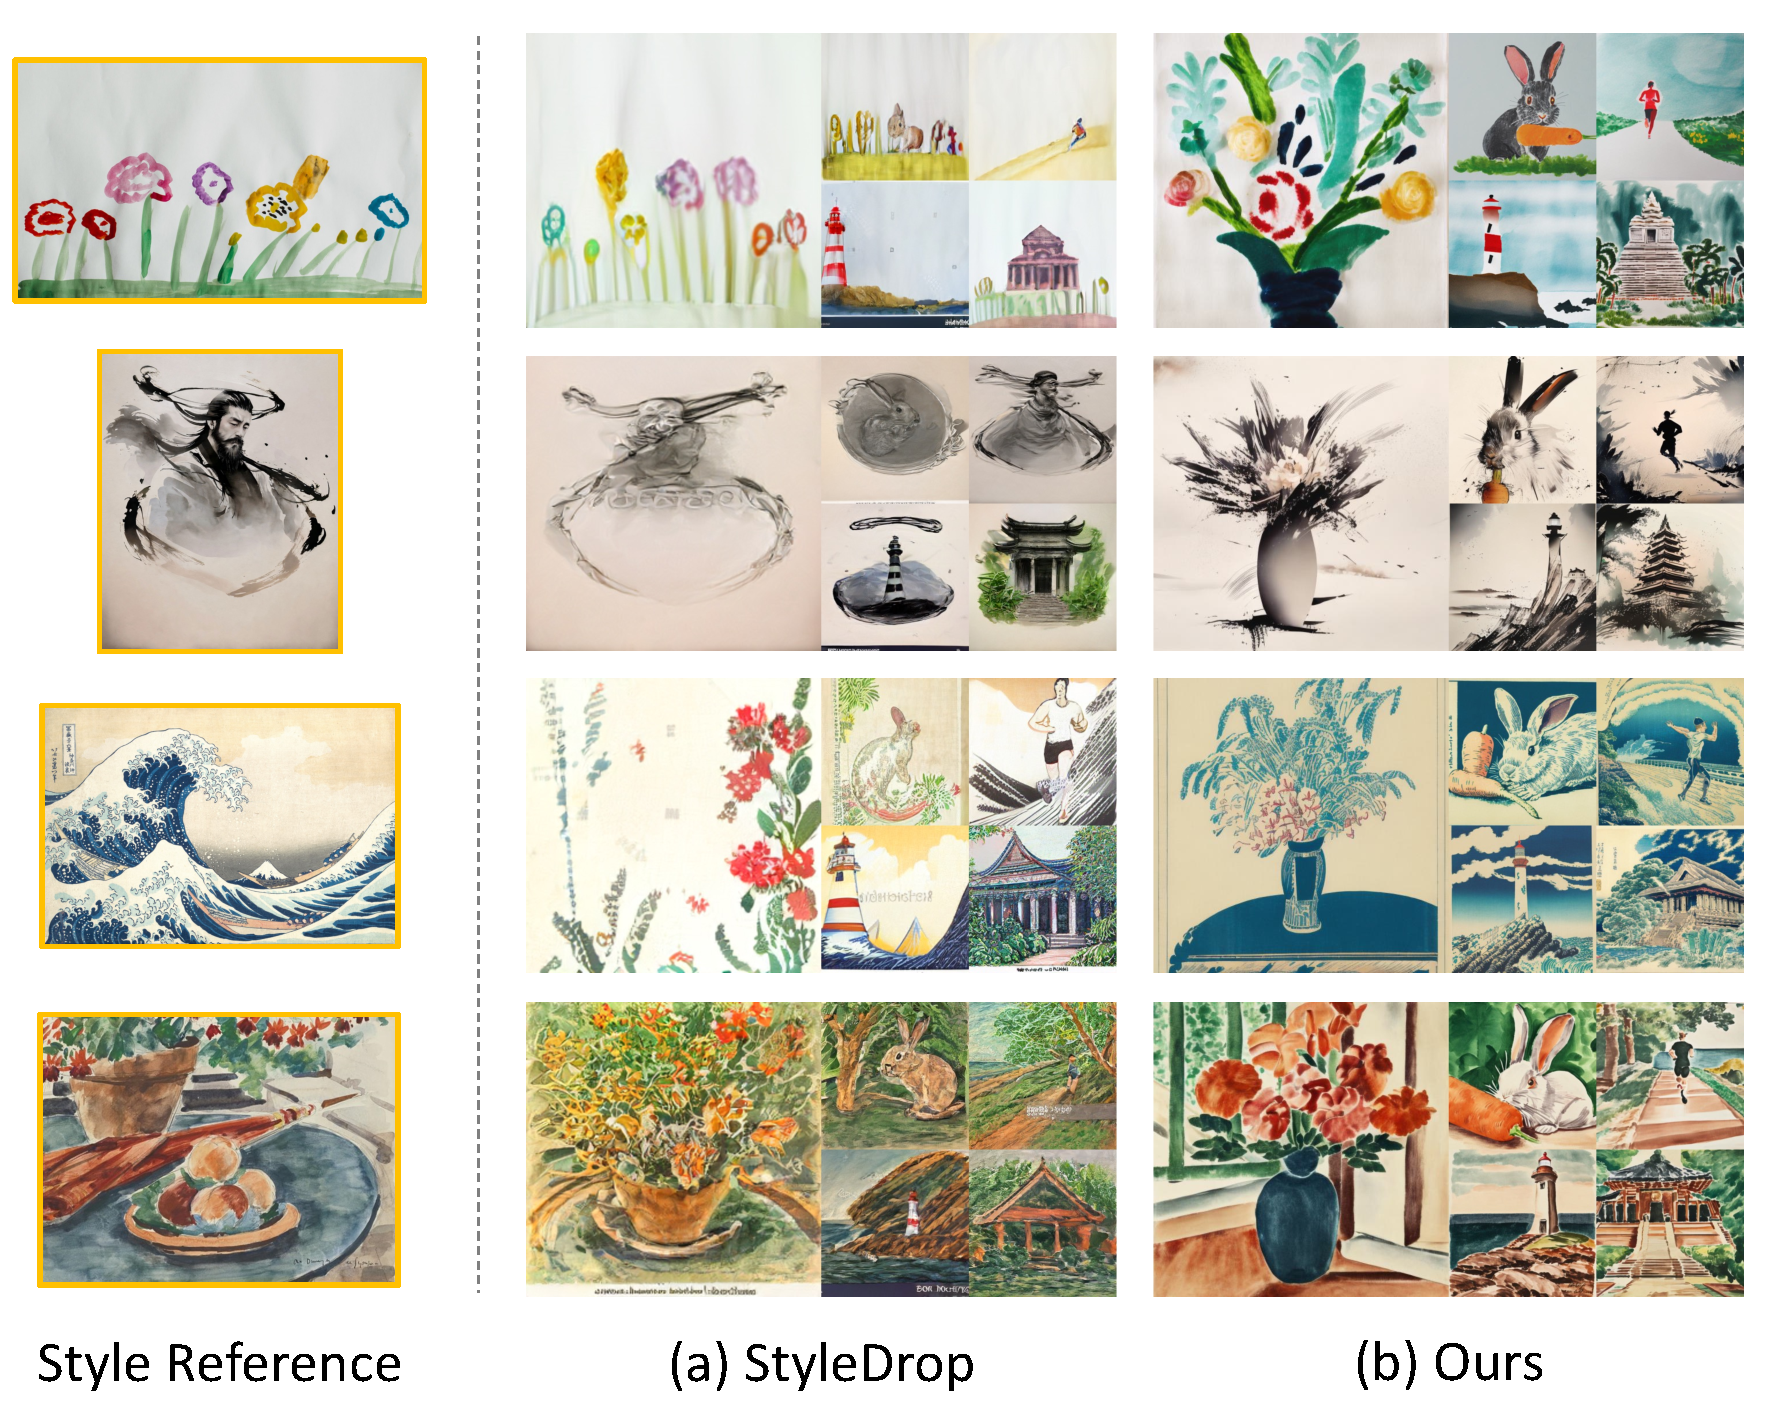
\includegraphics[width=0.8\linewidth]{figures/supp/result_comp_styledrop.pdf}
    \vspace{-1.2em}
    \caption{Visual comparison between StyleDrop and our proposed method. Testing prompts: (i) \textit{A woman reading a book in a park.}; (ii) \textit{A person jogging along a scenic trail.}; (iii) \textit{A colorful butterfly resting on a flower.}; (iv) \textit{A rabbit nibbling on a carrot.}; (v) \textit{A telescope pointed at the stars.}} 
    \label{fig:supp_comp_styledrop}
\end{figure}
%
\begin{table}[!h]
\centering
%\setlength{\tabcolsep}{3.0pt}
% \renewcommand\arraystretch{1.5}
% \vspace{-1em}
\caption{Quantitative comparison with StyleDrop.}
\vspace{-1em}
\label{tab:supp_comp_styledrop}
\resizebox{0.6\linewidth}{!}{
  \begin{tabular}{ccc} % {@{}lc@{}}
    % \toprule
    %  \hline
    %  & \multicolumn{5}{|c}{\textbf{CLIP scores}} \\
    \hline
    Methods & StyleDrop & Ours(SD 2.1) \\
    \hline
    \texttt{Text} $\uparrow$ & 0.2389 & 0.3028 \\
    \texttt{Style} $\uparrow$ & 0.3962 & 0.4836 \\
    \hline
  \end{tabular}
}
\end{table}

\subsection{Comparison with Style Transfer Methods}

In this section, we perform comparisons with a particular set of competitors, i.e., style transfer methods. As style transfer methods require extra source images or videos for content provision, we utilize text-to-image models(Stable Diffusion 2.1) and text-to-video models(VideoCrafter) to initially generate visual content. Subsequently, we apply existing style transfer methods based on the reference to produce the stylized output. For stylized image generation, we opt for T2I + CAST\cite{zhang2022domain}, while for stylized video generation, we choose T2V + MCCNet\cite{deng2021arbitrary}. The results of this comparison are illustrated in the Table~\ref{tab:supp_comp_cast} and Table~\ref{tab:supp_comp_mccnet}. 
Both two competitors underperform our approach.
The reasons are in two aspects: (i) Style transfer methods mainly work well on transferring tones and local textures while fall short in transferring semantic style features; (ii) Style transfer method cannot change the structure of the content image, which hinders the generation of styles that associated with special geometry features, e.g. layouts of logo style and 3D render style.

\begin{table}[!h]
\centering
%\setlength{\tabcolsep}{3.0pt}
% \renewcommand\arraystretch{1.5}
% \vspace{-1em}
\caption{Quantitative comparison with image style transfer method.}
\vspace{-1em}
\label{tab:supp_comp_cast}
%\resizebox{0.6\linewidth}{!}{
  \begin{tabular}{ccc} % {@{}lc@{}}
    % \toprule
    %  \hline
    %  & \multicolumn{5}{|c}{\textbf{CLIP scores}} \\
    \hline
    Methods & T2I + CAST & Ours(SD 2.1) \\
    \hline
    \texttt{Text} $\uparrow$ & 0.3027 & 0.3028 \\
    \texttt{CLIP-Style} $\uparrow$ & 0.3549 & 0.4836 \\
    % \texttt{DINO-Style} $\uparrow$ & 0.2645 & 0.3652 \\
    \hline
  \end{tabular}
% }
\end{table}

\begin{table}[!h]
\centering
%\setlength{\tabcolsep}{3.0pt}
% \renewcommand\arraystretch{1.5}
% \vspace{-1em}
\caption{Quantitative comparison with video style transfer method.}
\vspace{-1em}
\label{tab:supp_comp_mccnet}
% \resizebox{0.6\linewidth}{!}{
  \begin{tabular}{ccc} % {@{}lc@{}}
    % \toprule
    %  \hline
    %  & \multicolumn{5}{|c}{\textbf{CLIP scores}} \\
    \hline
    Methods & T2I + MCCNet & Ours(VideoCrafter) \\
    \hline
    \texttt{Text} $\uparrow$ & 0.2487 & 0.2726 \\
    \texttt{Style} $\uparrow$ & 0.2858 & 0.4531 \\
    \texttt{Temporal} $\uparrow$ & 0.9577 & 0.9892 \\
    \hline
  \end{tabular}
% }
\end{table}


%%%%%%%%%%%%%%%%%%%%%%%%%%%%%%%%%
\section{Extended Ablation Study}
\label{sec:supp_extend_ablation}
% \addcontentsline{toc}{chapter}{D. Extended Ablation Study}

Since we have made ablation studies on some key design in the main text(i.e., Dual Cross-Attention, Data Augmentation, and Adaptive Style-Content Fusion), we provide additional comparison between different style adapter architechures, including MLP, Transformer, and Query Transformer(ours). Quantitative results and visual comparisons in Figure \ref{fig:supp_ablation_arch} and Table \ref{tab:supp_ablation_arch} show that Query Transformer excels over the other alternatives.

\begin{table}[!h]
% \vspace{-1em}
\centering
\caption{Ablation studies on style feature extractor architecture. The performance is evaluated on the style-guided T2I generation.}
\label{tab:supp_ablation_arch}
\vspace{-1em}
% \renewcommand\arraystretch{1.2}
  \begin{tabular}{cccc} % {@{}lc@{}}
    % \toprule
    \hline
    Alternatives & MLP & Transformer & Q-Former (Ours) \\
    \hline
    Text $\uparrow$ & 0.3415 & 0.3221 & 0.3028 \\
    Style $\uparrow$ & 0.2843 & 0.4149 & 0.4836 \\
    \hline
  \end{tabular}
  
\end{table}

\begin{figure}[h]
    \centering
    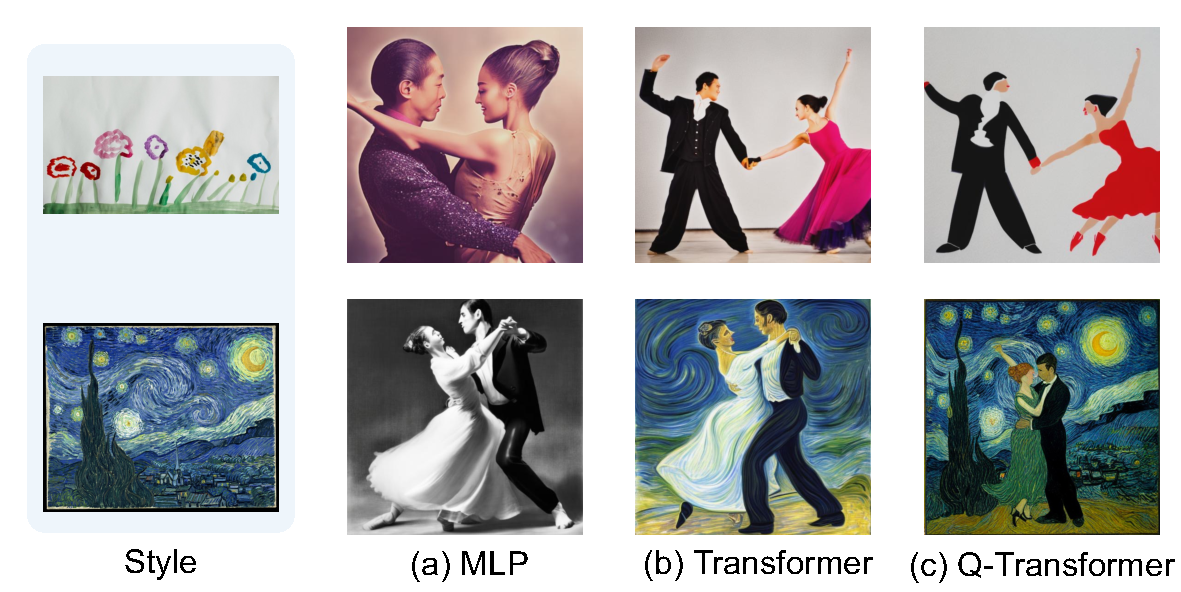
\includegraphics[width=\linewidth]{figures/supp/ablation_arch.pdf}
    \vspace{-1em}
    \caption{Visual comparison between different adapter architectures. Prompt: \textit{A couple dancing gracefully together.}}
    \label{fig:supp_ablation_arch}
\end{figure}

%%%%%%%%%%%%%%%%%%%%%%%%%%%%%%%%%
\section{Application Extension}
\label{sec:supp_app}


In this section, we further explore the compatibility with additional controllable conditions, e.t., depth. Following the approach of structure control in Animate-A-Story\cite{he2023animate}, we introduce video structure control by integrating a well-trained depth adapter into the base T2V model. Note that StyleCrafter and depth-adapter are trained independently, the only operation we take is to combine the both during the inference stage. Instead of employing DDIM Inversion to ensure consistency, we generate the videos from random noise. The visual comparison with VideoComposer\cite{wang2024videocomposer} is present in Figure~\ref{fig:supp_depth}. VideoComposer struggles to produce results faithful to text descriptions when faced with artistic styles, such as the "boat" mentioned in the prompt. In contrast, our method not only supports collaboration with depth guidance, but also generates videos with controllable content, style, and structure. 


% %%%%%%%%%%%%%%%%%%%%%%%%%%%%%%%%%
% \section{Further Exploration}
% \TODO{(11.23-11.24) We have explored an enhanced version trained with a few stylized videos.}

%%%%%%%%%%%%%%%%%%%%%%%%%%%%%%%%%
\section{More Results}
\label{sec:supp_more_result}

In this section, we provide more visual results and comparisons of our method. Specifically, we provide: (i) style-guided text-to-image generation results on StyleCrafter(SD2) and StyleCrafter(SDXL) in Figure~\ref{fig:supp_more_result_img_sd} and Figure~\ref{fig:supp_more_result_img_sdxl}; (ii) comparison of single-reference stylized video generation and multi-reference stylized video generation, as illustrated in Figure~\ref{fig:supp_more_result_comp_single} and Figure~\ref{fig:supp_more_result_comp_multi}, respectively. (iii) additional stylized video results in Figure~\ref{fig:supp_more_result_ours_1} and Figure~\ref{fig:supp_more_result_ours_2}.


%\clearpage

\section{Limitations}
\label{sec:supp_limitation}

While our proposed method effectively handles most common styles, it does have certain limitations. Firstly, since StyleCrafter is developed based on existing T2I models and T2V models, such as SDXL and VideoCrafter, it unavoidably inherits part of the base model's shortcomings, such as fixed resolution and video length, less satisfactory temporal consistency. For example, our method fails to generate high-definition faces in certain cases, as shown in Figure~\ref{fig:supp_failure}. Despite the fact that our approach successfully enhances the stylistic generation capacity of T2I/T2V models, leveraging a powerful base model will always amplify its performance, as showcased in the superior style conformity of StyleCrafter(SDXL) over StyleCrafter(SD2).

Besides, artistic style is a very comprehensive perceptual feeling and visual styles are considerably more complex than what we explore in our paper. Our model may produce just passable results when confronted with reference images possessing highly stylized semantics. For example, as depicted in Figure~\ref{fig:supp_failure}, although our model successfully reproduces ink strokes, there are still discrepancies with reference images in the aesthetic level, such as the lack of "blank-leaving" in the generation results. Additionally, considering the absence of stylized video data, our stylized video generation results are somewhat less satisfactory than stylized image generation in visual style expression. A possible solution is to collect sufficient stylized video data for training, which we leave for further work. 


%
\begin{figure}[!h]
    \centering
    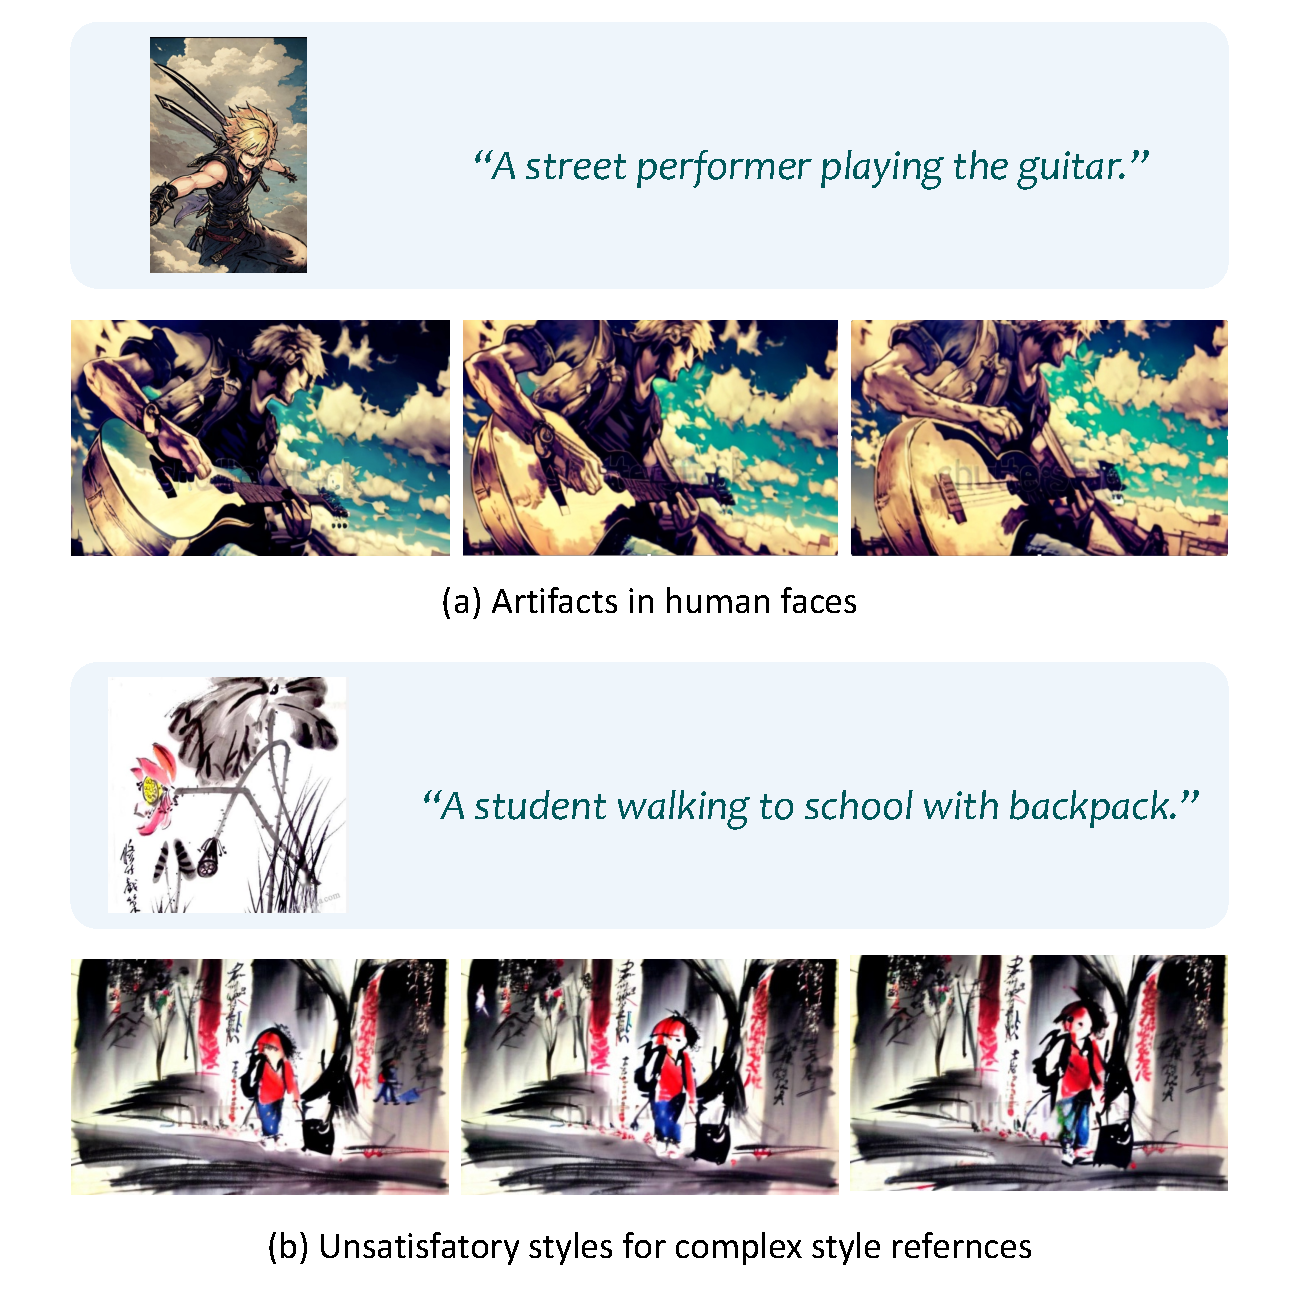
\includegraphics[width=\linewidth]{figures/supp/limit.pdf}
    \caption{Failure cases of our methods. (a). Our method inherits limitations from the pretrained T2V model, tends to generate human faces with obvious artifacts. (b). Our method produces less satisifactory styles for complex style references such as Chinese Ink Painting.} 
    \label{fig:supp_failure}
\end{figure}


\begin{figure*}[p]
    \vspace*{\fill}
    \centering
    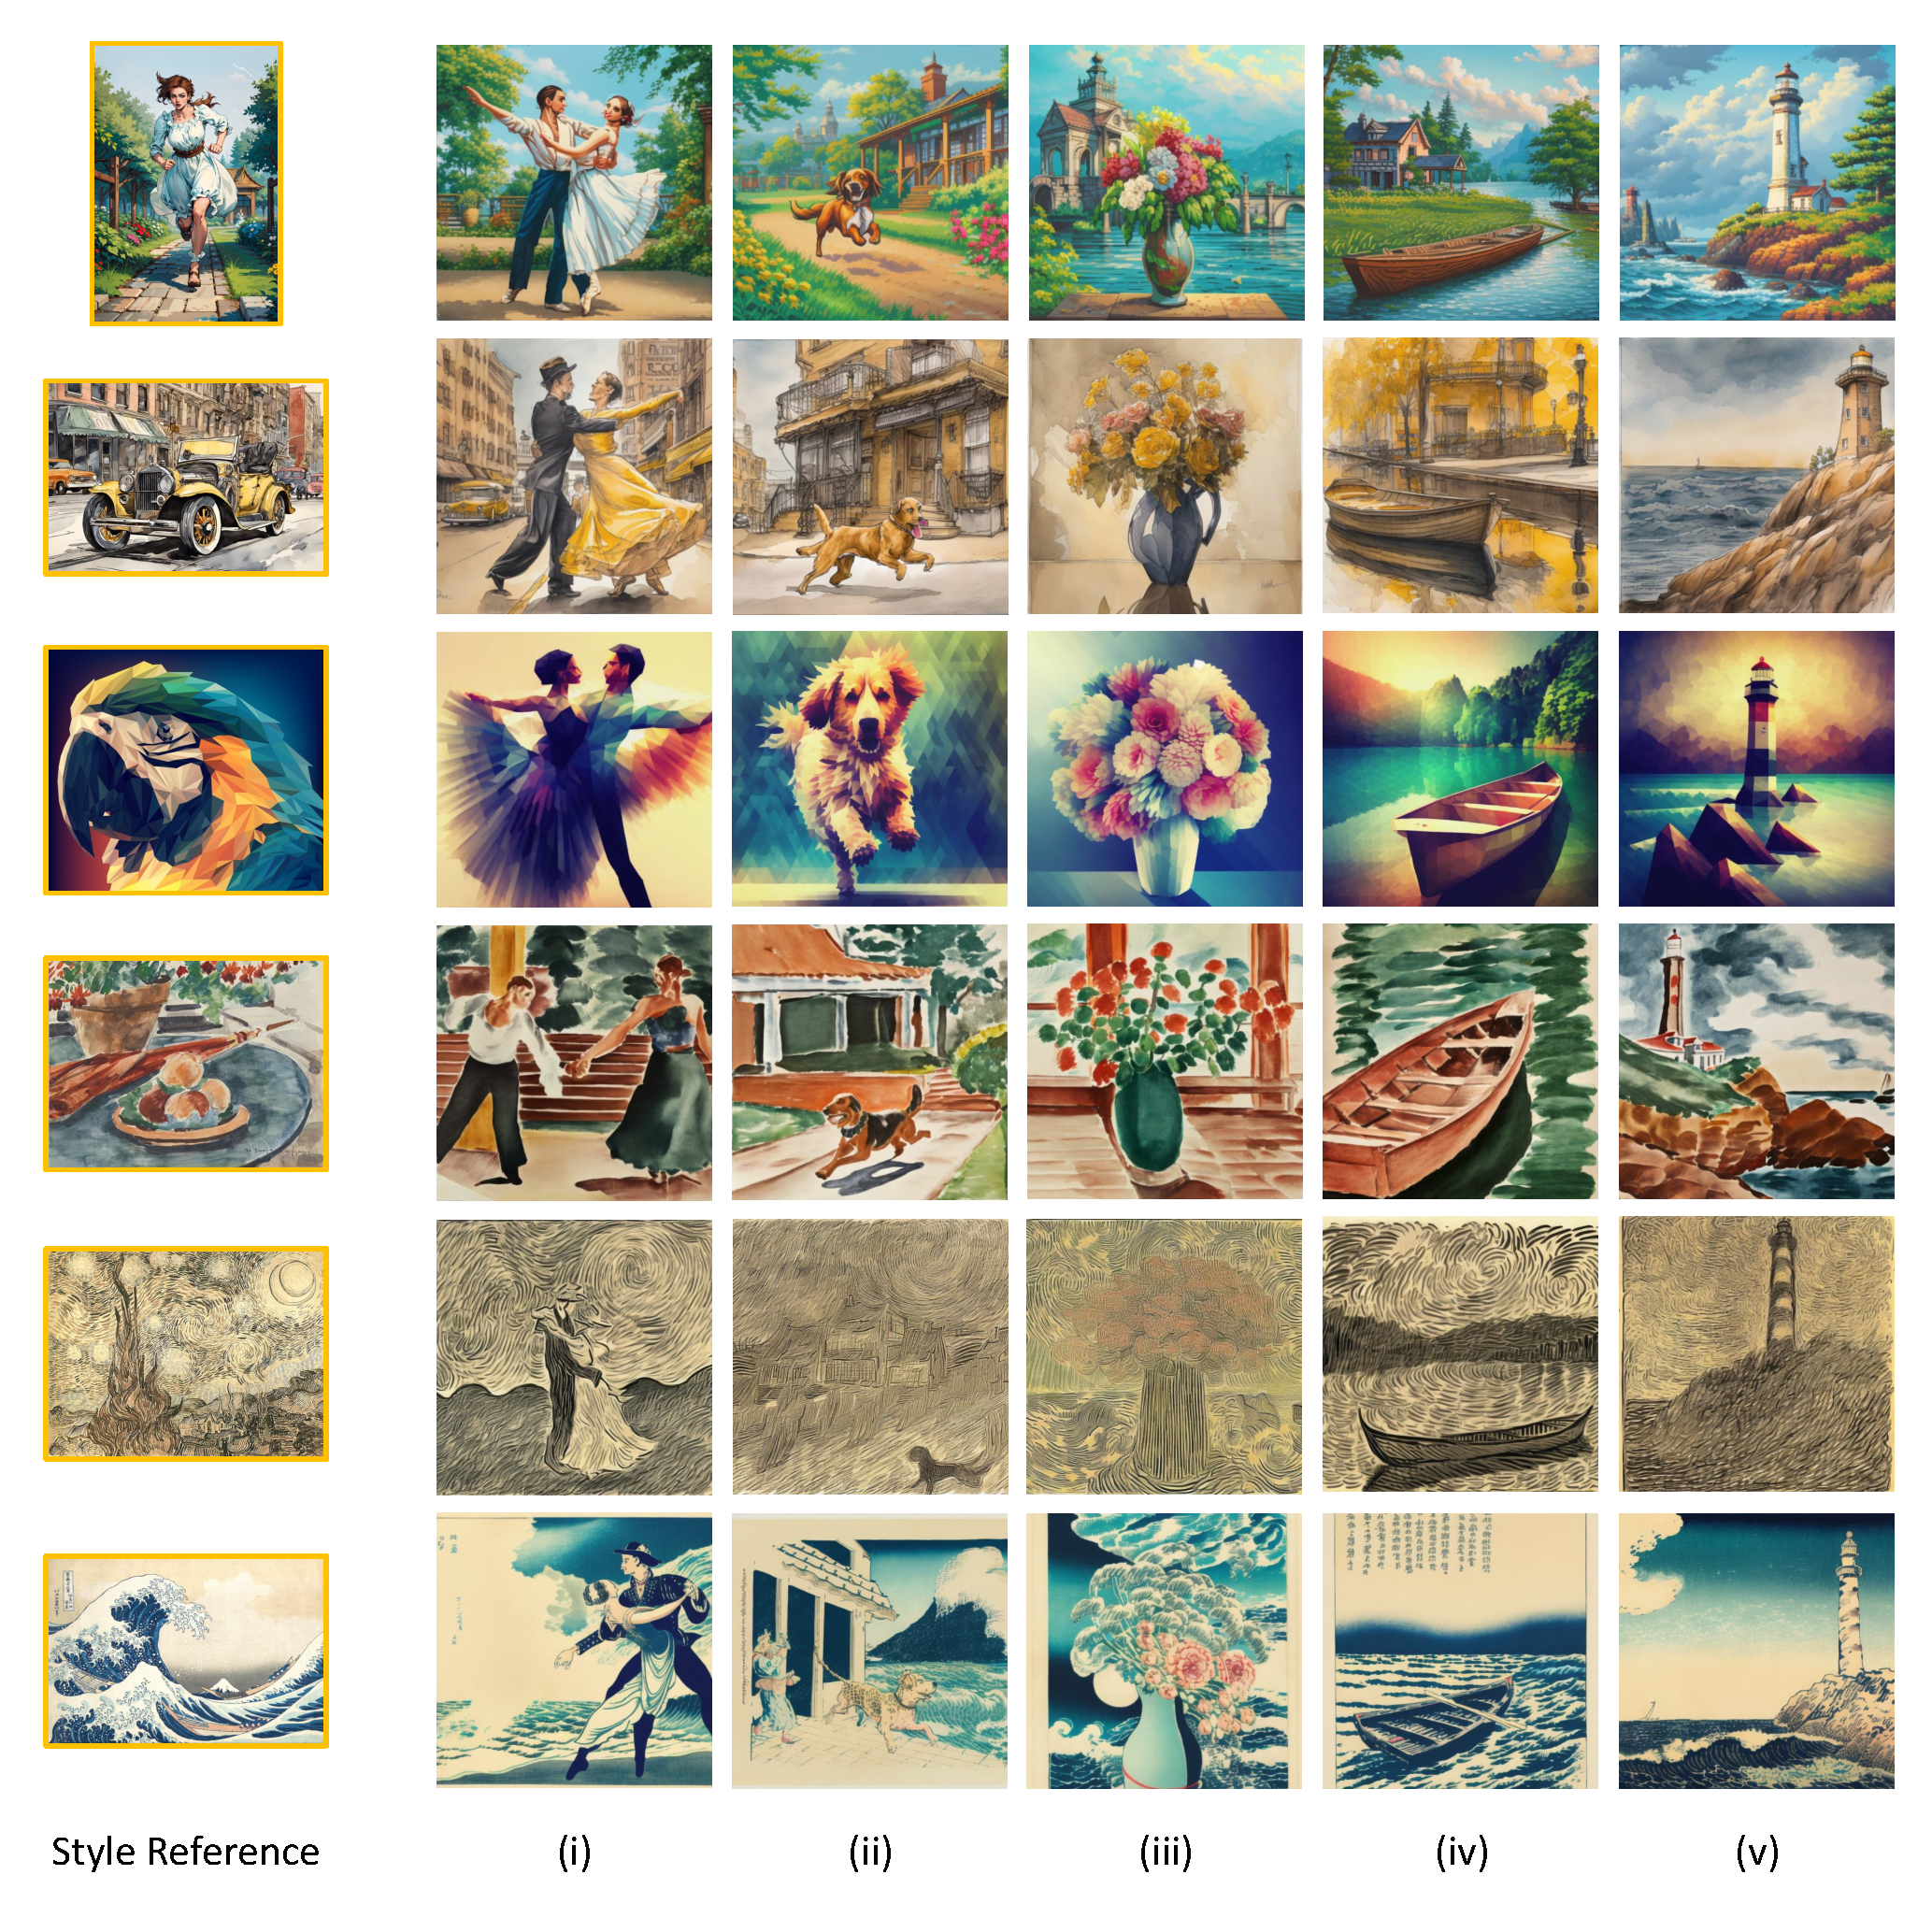
\includegraphics[width=\linewidth]{figures/supp/more_results_img_sd.pdf}
    \caption{More Results of \textbf{StyleCrafter(SD2)} on Style-Guided Text-to-Image Generation. Prompts: (i) A couple dancing gracefully together. (ii) A dog is running in front of a house. (iii) A bouquet of flowers in a vase. (iv) A rowboat docked on a peaceful lake. (v) A lighthouse standing tall on a rocky coast.} 
    \label{fig:supp_more_result_img_sd}
    \vspace*{\fill}
\end{figure*}

\begin{figure*}[p]
    \vspace*{\fill}
    \centering
    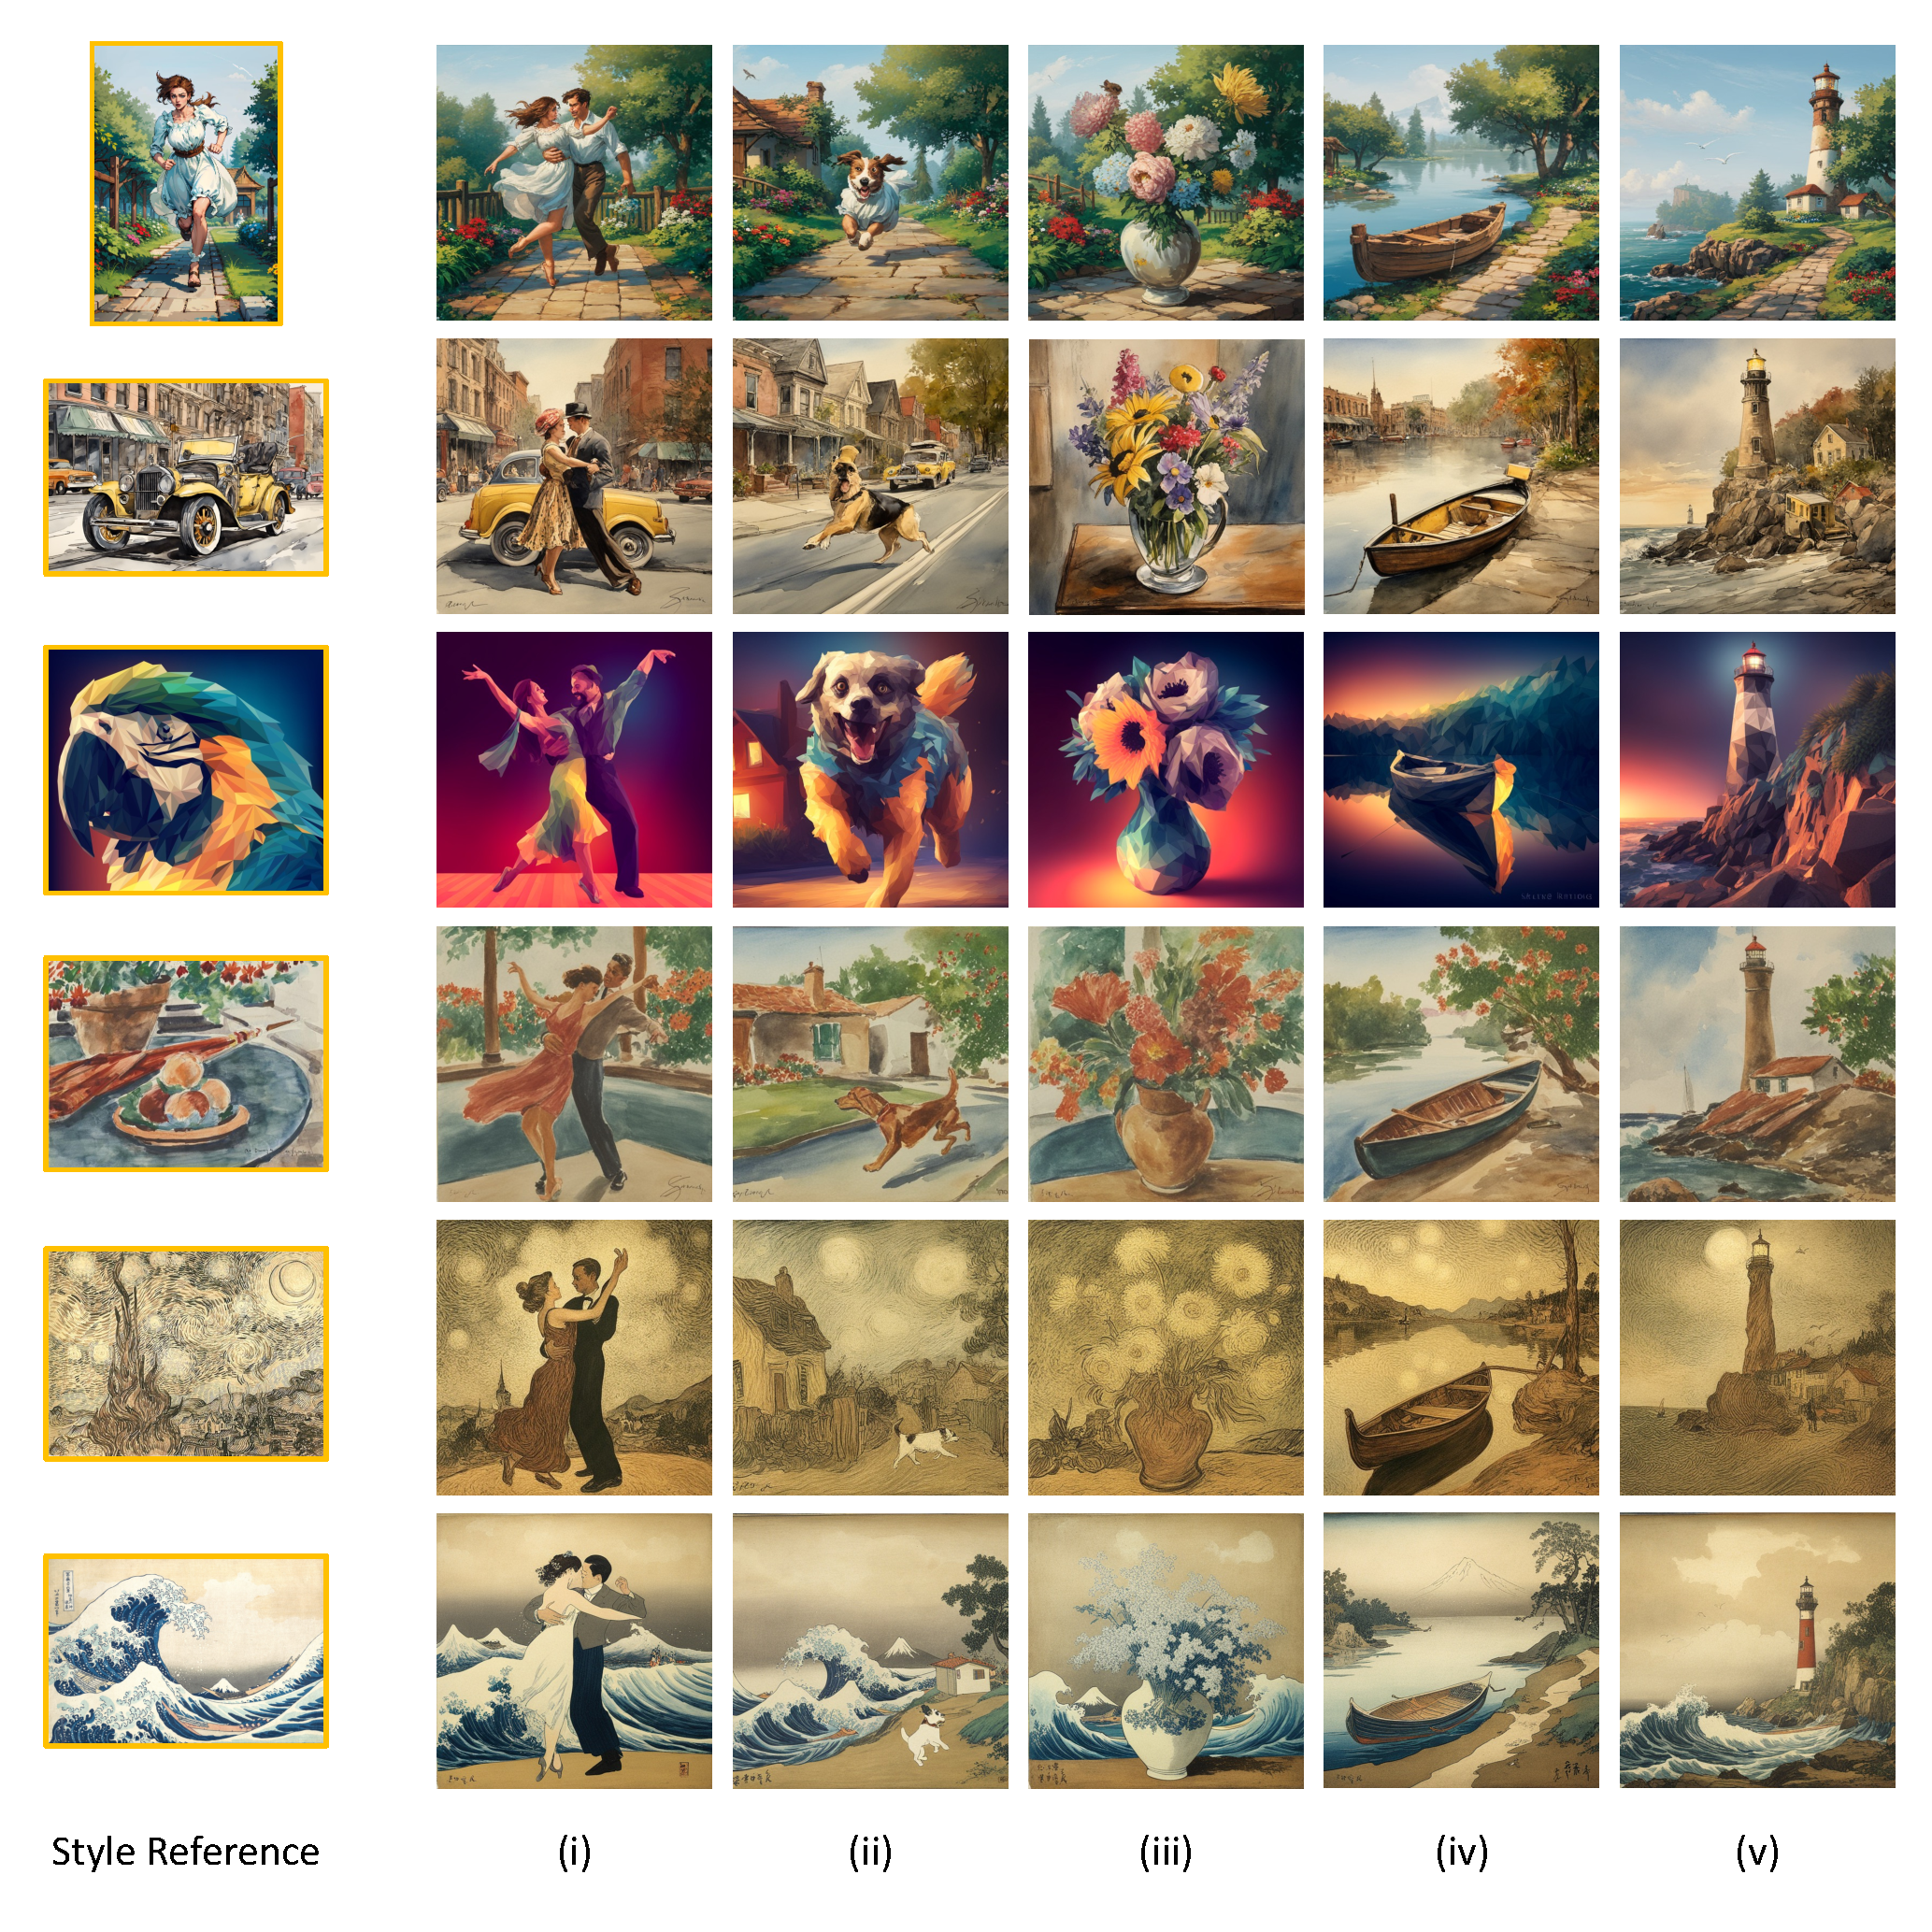
\includegraphics[width=\linewidth]{figures/supp/more_results_img_sdxl.pdf}
    \caption{More Results of \textbf{StyleCrafter(SDXL)} on Style-Guided Text-to-Image Generation. Prompts: (i) A couple dancing gracefully together. (ii) A dog is running in front of a house. (iii) A bouquet of flowers in a vase. (iv) A rowboat docked on a peaceful lake. (v) A lighthouse standing tall on a rocky coast.} 
    \label{fig:supp_more_result_img_sdxl}
    \vspace*{\fill}
\end{figure*}


\begin{figure*}[t]
    \centering
    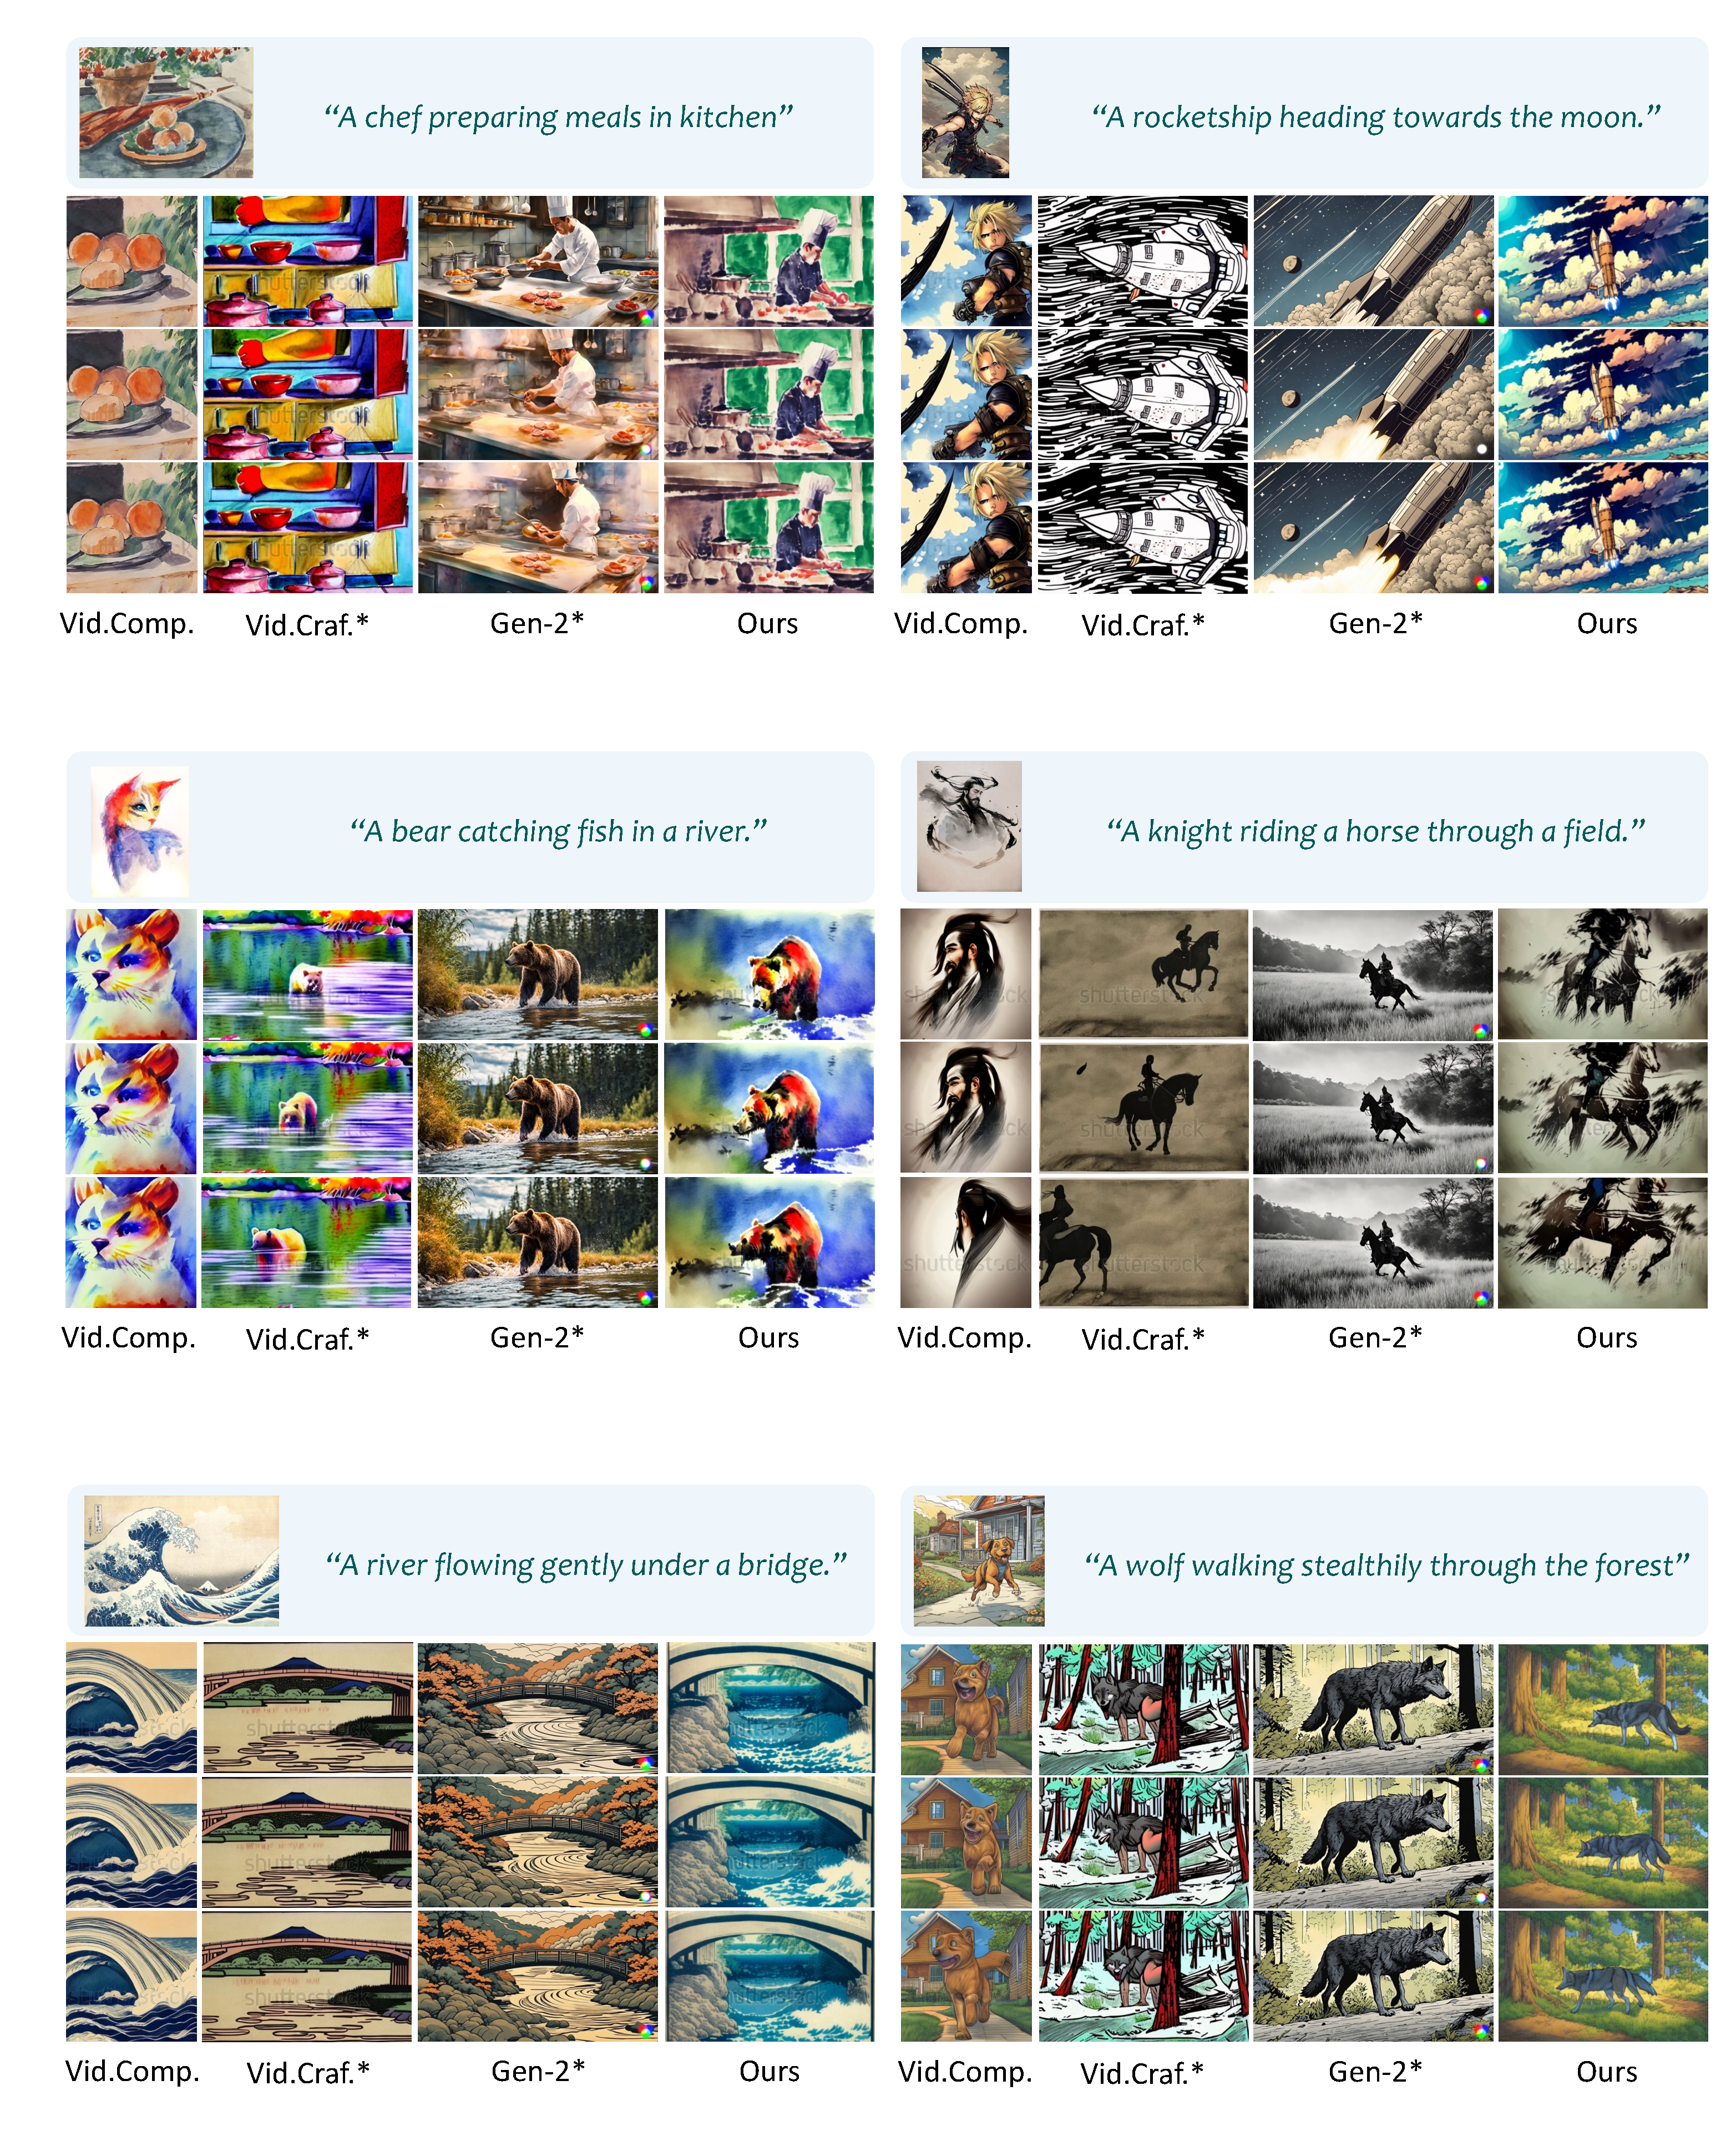
\includegraphics[width=0.9\linewidth]{figures/supp/result_comp_single_ref_1.pdf}
    \caption{More Visual Comparison on Sinlge-Reference Stylized T2V Generation. Vid.Comp.: VideoComposer; Vid.Craf.: VideoCrafter.} 
    \label{fig:supp_more_result_comp_single}
\end{figure*}

\begin{figure*}[t]
    \centering
    \vspace{-1.5em}
    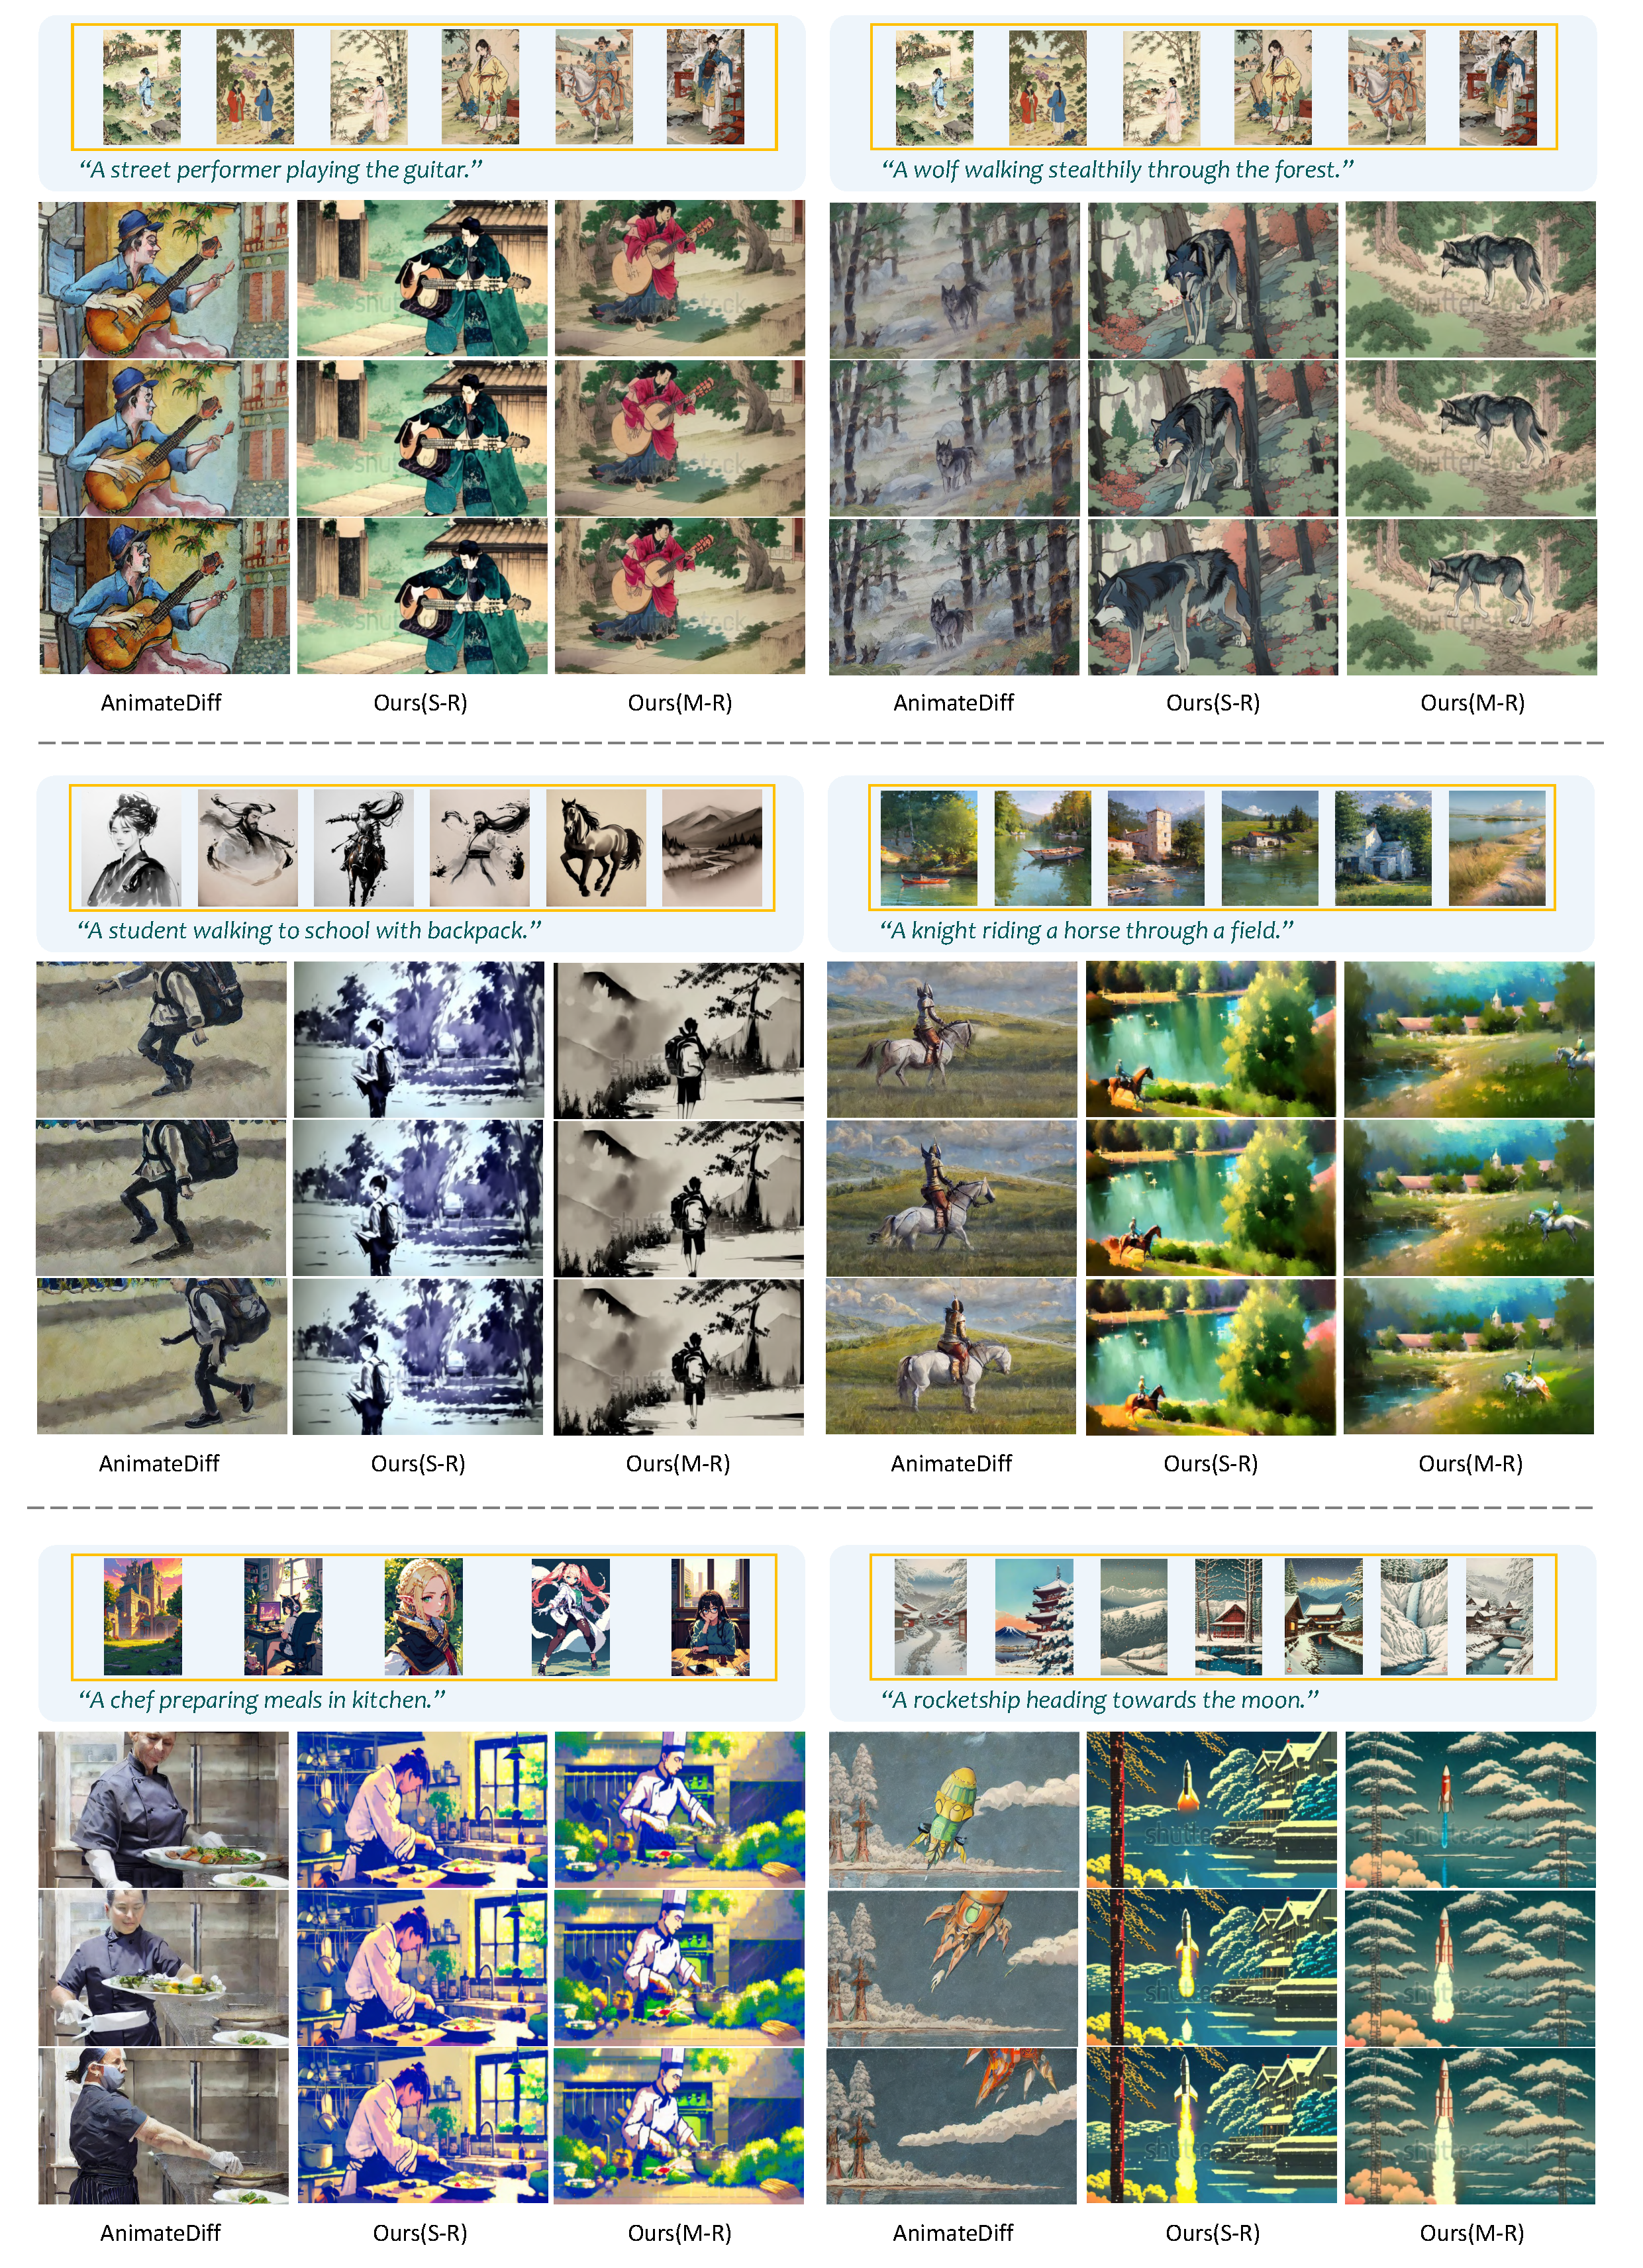
\includegraphics[width=0.85\linewidth]{figures/supp/result_comp_multi_ref_vid.pdf}
    \vspace{-0.8em}
    \caption{More Visual Comparison on Multi-Reference Stylized T2V Generation} 
    \label{fig:supp_more_result_comp_multi}
\end{figure*}


\begin{figure*}[t]
    \centering
    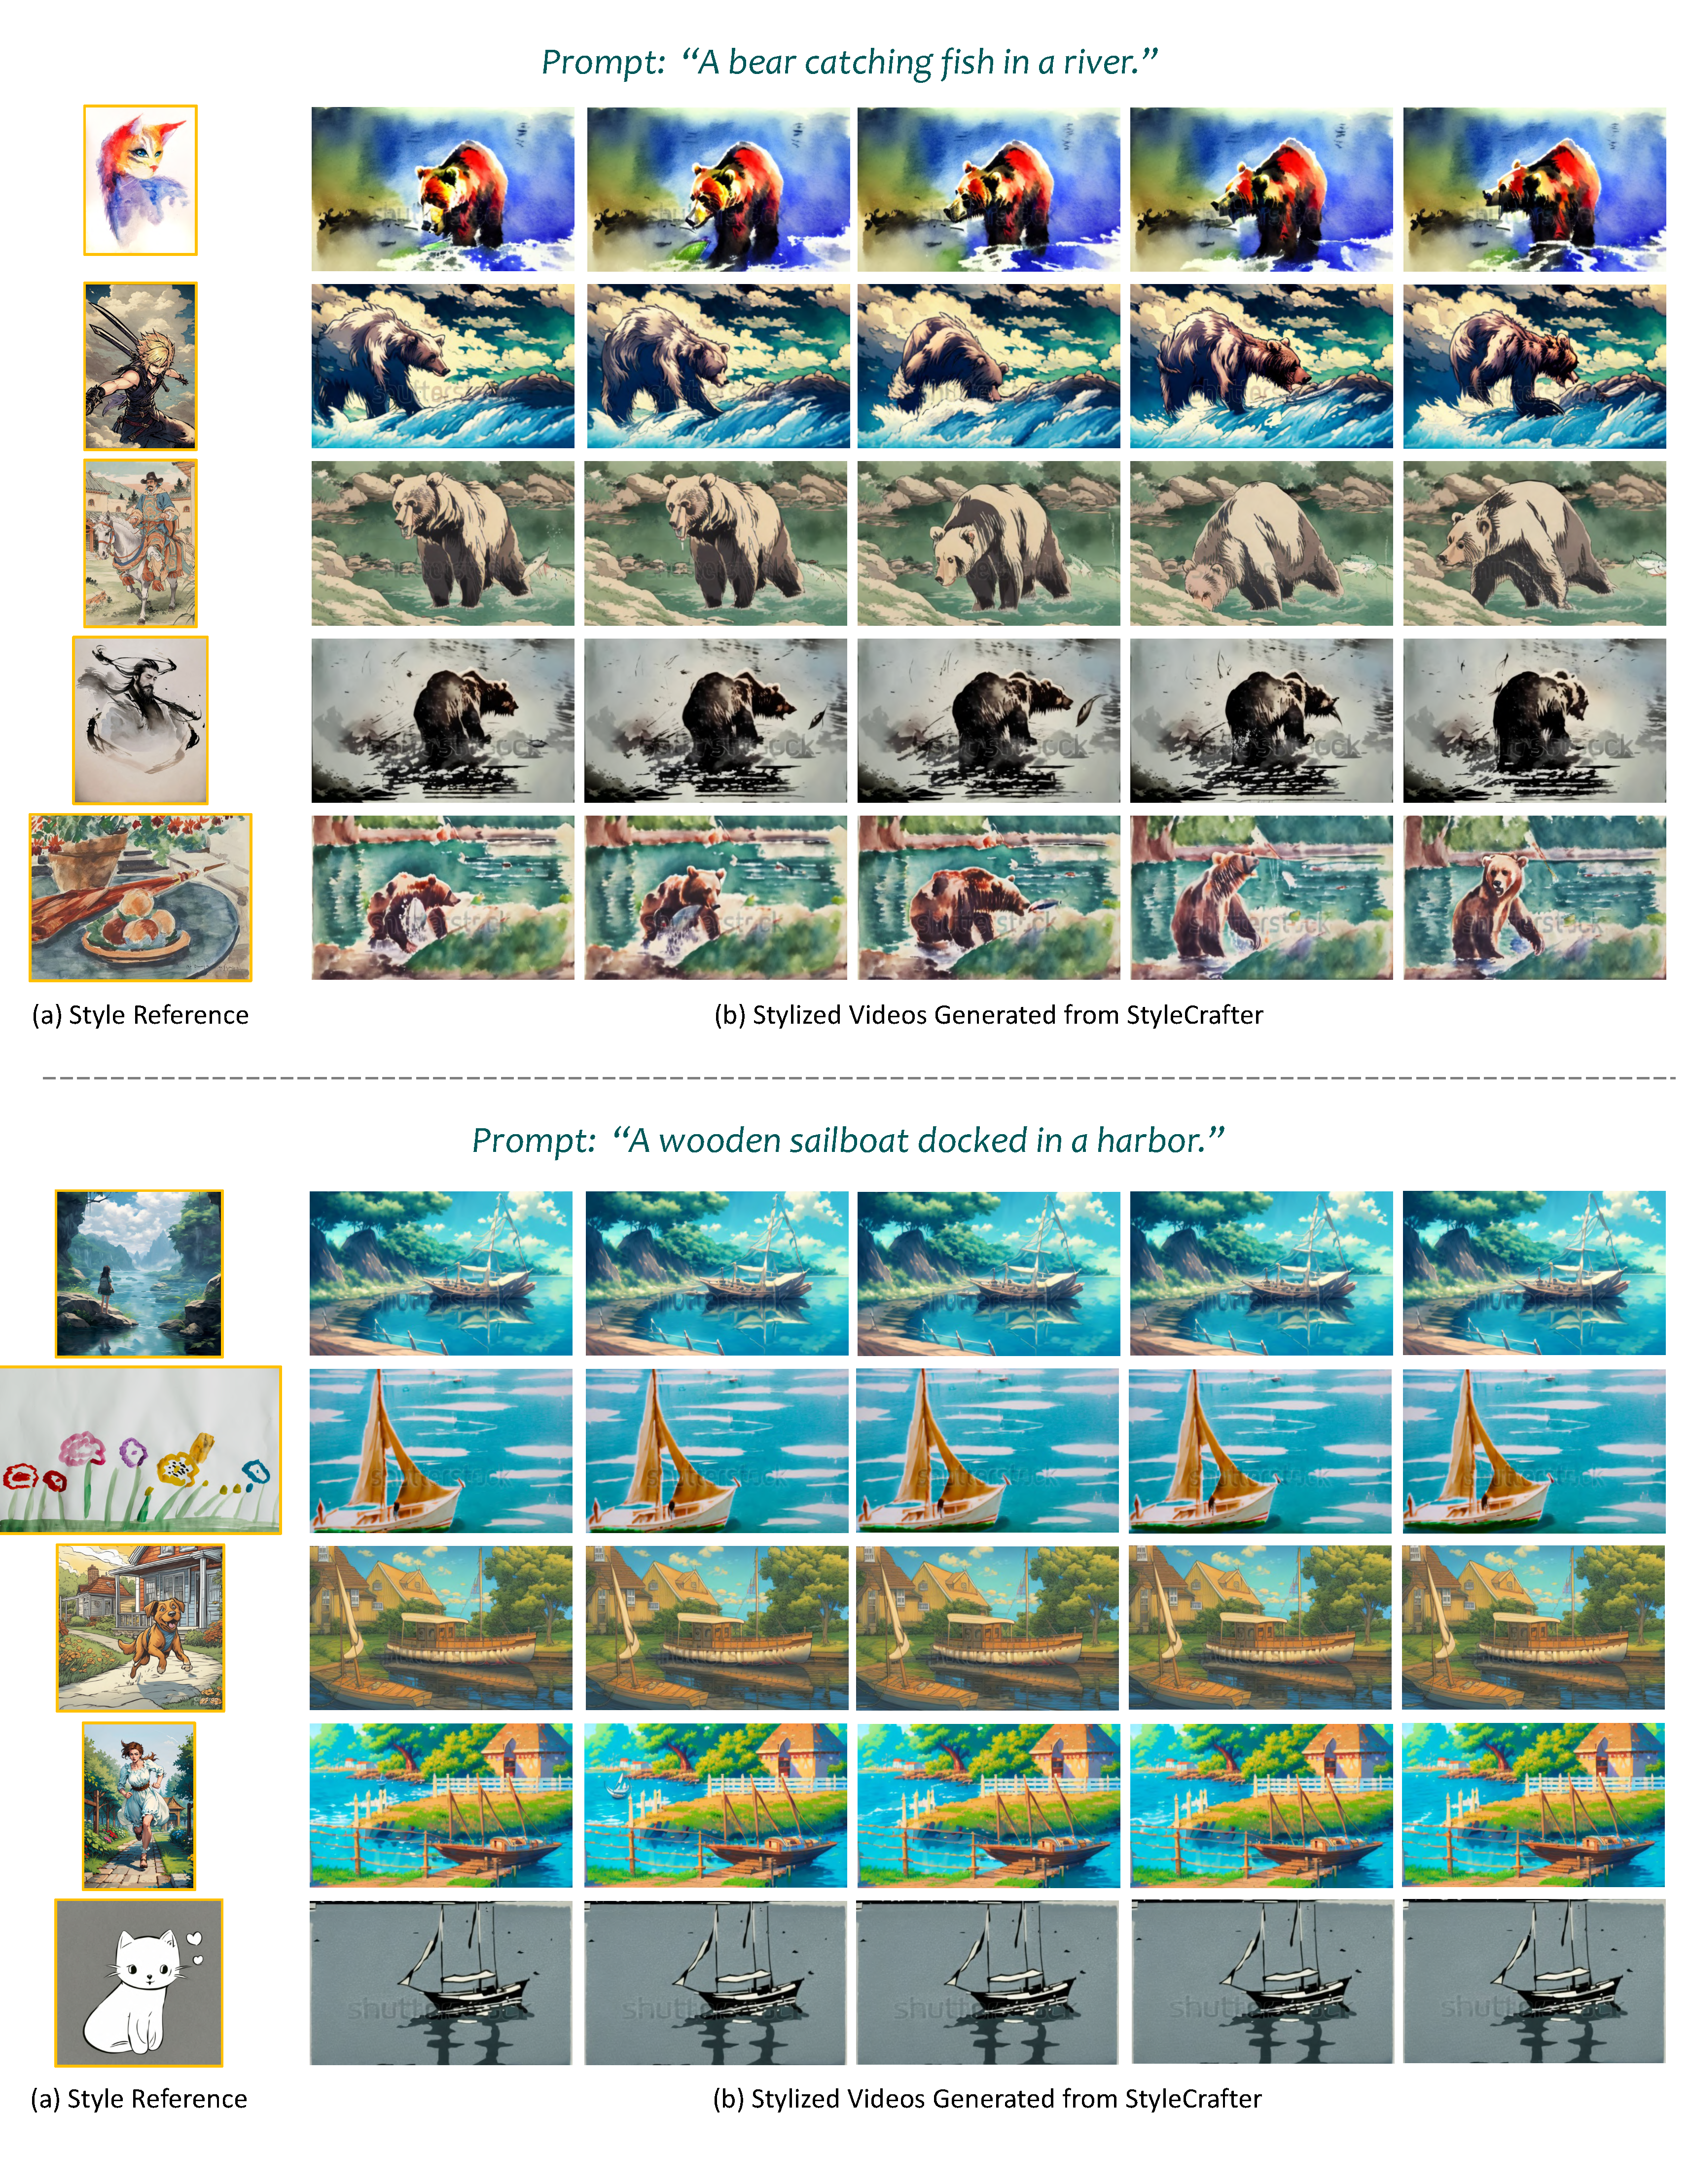
\includegraphics[width=0.9\linewidth]{figures/supp/result_ours_1.pdf}
    \vspace{-1.5em}
    \caption{More Results of StyleCrafter on Style-Guided Text-to-Video Generation} 
    \label{fig:supp_more_result_ours_1}
\end{figure*}

\begin{figure*}[t]
    \centering
    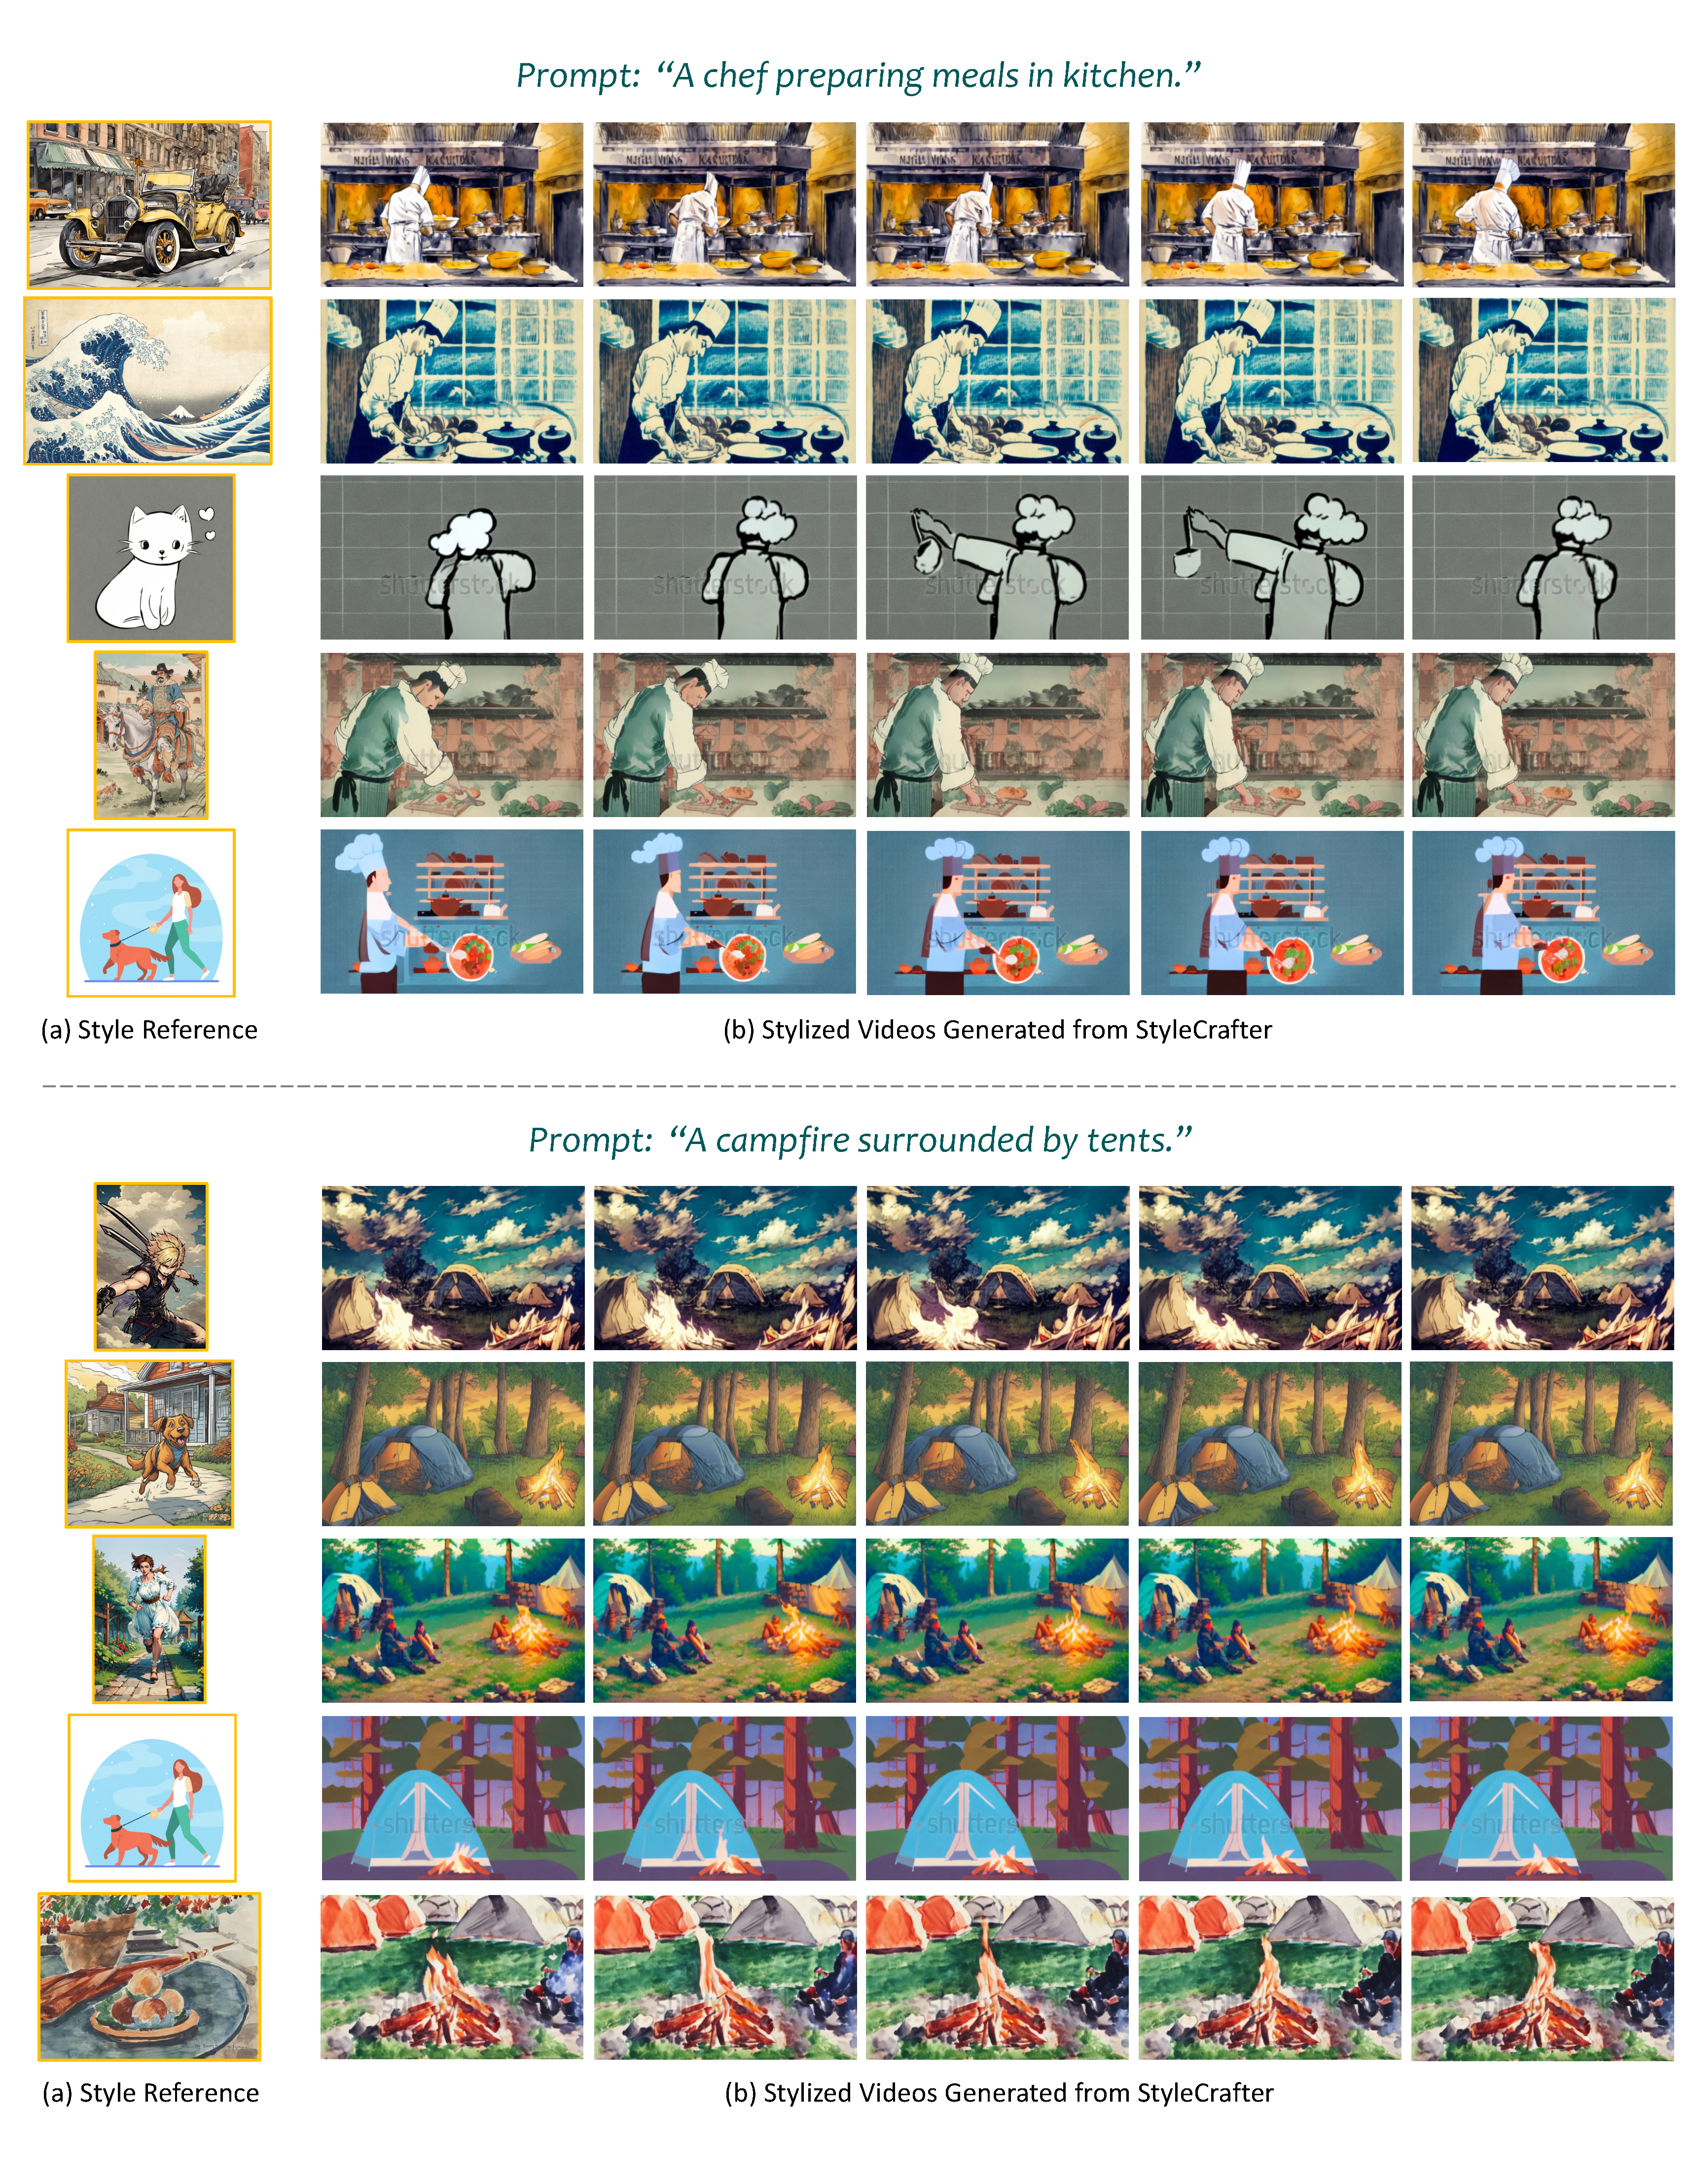
\includegraphics[width=0.9\linewidth]{figures/supp/result_ours_2.pdf}
    \vspace{-1em}
    \caption{More Results of StyleCrafter on Style-Guided Text-to-Video Generation} 
    \label{fig:supp_more_result_ours_2}
\end{figure*}


